\documentclass[
  digital,     %% The `digital` option enables the default options for the
               %% digital version of a document. Replace with `printed`
               %% to enable the default options for the printed version
               %% of a document.
%%  color,       %% Uncomment these lines (by removing the %% at the
%%               %% beginning) to use color in the printed version of your
%%               %% document
  oneside,     %% The `oneside` option enables one-sided typesetting,
               %% which is preferred if you are only going to submit a
               %% digital version of your thesis. Replace with `twoside`
               %% for double-sided typesetting if you are planning to
               %% also print your thesis. For double-sided typesetting,
               %% use at least 120 g/m² paper to prevent show-through.
  nosansbold,  %% The `nosansbold` option prevents the use of the
               %% sans-serif type face for bold text. Replace with
               %% `sansbold` to use sans-serif type face for bold text.
  nocolorbold, %% The `nocolorbold` option disables the usage of the
               %% blue color for bold text, instead using black. Replace
               %% with `colorbold` to use blue for bold text.
  lof,         %% The `lof` option prints the List of Figures. Replace
               %% with `nolof` to hide the List of Figures.
  lot,         %% The `lot` option prints the List of Tables. Replace
               %% with `nolot` to hide the List of Tables.
]{fithesis4}
%% The following section sets up the locales used in the thesis.
\usepackage[resetfonts]{cmap} %% We need to load the T2A font encoding
\usepackage[
  main=english, %% By using `czech` or `slovak` as the main locale
                %% instead of `english`, you can typeset the thesis
                %% in either Czech or Slovak, respectively.
  % english, german, russian, czech, slovak %% The additional keys allow
]{babel}        %% foreign texts to be typeset as follows:
%%
%%   \begin{otherlanguage}{german}  ... \end{otherlanguage}
%%   \begin{otherlanguage}{russian} ... \end{otherlanguage}
%%   \begin{otherlanguage}{czech}   ... \end{otherlanguage}
%%   \begin{otherlanguage}{slovak}  ... \end{otherlanguage}
%%
%% For non-Latin scripts, it may be necessary to load additional
%% fonts:
\usepackage{paratype}
% \def\textrussian#1{{\usefont{T2A}{PTSerif-TLF}{m}{rm}#1}}
%%
%% The following section sets up the metadata of the thesis.
\thesissetup{
  % * ✅
    date        = \the\year/\the\month/\the\day,
    university  = mu,
    faculty     = fi,
    type        = bc,
    department  = Department of Computer Systems and Communications,
    author      = Dominik Tichý,
    gender      = m,
    advisor     = {RNDr. Tomáš Raček, Ph.D.},
    title       = {Modern visualization of partial atomic charges in Mol*},
    TeXtitle    = {Modern visualization of partial atomic charges in Mol*},
    % * ✅
    keywords    = {%
        Mol*,
        ACC~II,
        αCharges,
        AlphaFold,
        SB NCBR,
        partial atomic charges,
        molecular visualization,
        chemical file formats,
        structural biology
    },
    TeXkeywords = {%
        Mol*,
        ACC~II,
        αCharges,
        AlphaFold,
        SB NCBR,
        partial atomic charges,
        molecular visualization,
        chemical file formats,
        structural biology
    },
    % * ✅
    abstract    = {%
      Partial atomic charges play a crucial role in computational chemistry as they help describe a molecule's electron density, providing essential insights into its properties.
      
      Visualizing these partial atomic charges was previously done using the Litemol viewer. However, the Litemol viewer is no longer maintained, and its replacement, the Mol* viewer, currently lacks support for visualizing partial atomic charges.
      
      This thesis addresses this gap in functionality by extending the Mol* viewer to support the visualization of partial atomic charges. The extended Mol* viewer is subsequently integrated into the Atomic Charge Calculator II and αCharges web applications. In addition, the functionality of the Atomic Charge Calculator II application was upgraded to permit multiple calculations within a single request.
      
      These advancements provide researchers with enhanced visualization capabilities and user interfaces for calculating and analyzing partial atomic charges.
    },
    % * ✅
    thanks      = {%
      I would like to thank my advisor RNDr. Tomáš Raček, Ph.D. for his advice and guidance throughout the writing of this thesis. I would also like to thank my family and friends for their love and support.
    },
    % * ✅
    bib         = {%
        main.bib,
    },
    %% Remove the following line to use the JVS 2018 faculty logo.
    facultyLogo = fithesis-fi,
}
\usepackage{tipa}
\usepackage{makeidx}      %% The `makeidx` package contains
\makeindex                %% helper commands for index typesetting.
%% These additional packages are used within the document:
\usepackage{paralist} %% Compact list environments
\usepackage{amsmath}  %% Mathematics
\usepackage{amsthm}
\usepackage{amsfonts}
\usepackage{url}      %% Hyperlinks
\usepackage{markdown} %% Lightweight markup
\usepackage{listings} %% Source code highlighting
\lstset{
  basicstyle      = \ttfamily,
  identifierstyle = \color{black},
  keywordstyle    = \color{blue},
  keywordstyle    = {[2]\color{cyan}},
  keywordstyle    = {[3]\color{olive}},
  stringstyle     = \color{teal},
  commentstyle    = \itshape\color{magenta},
  breaklines      = true,
}
\usepackage{floatrow} %% Putting captions above tables
\floatsetup[table]{capposition=top}
\usepackage[babel]{csquotes} %% Context-sensitive quotation marks
\usepackage{minted}
\usepackage{subfigure}
\usepackage{textalpha}
\usepackage{dirtree}
\usepackage[export]{adjustbox}
\usepackage{pdfpages}
\usepackage{chemfig}
\usepackage{listings}
\usepackage[titletoc]{appendix}

\begin{document}

% * ✅
\newpage
\chapter*{Introduction}
\markright{\textsc{Introduction}}
\addcontentsline{toc}{chapter}{Introduction}
\label{chap:introduction}

Partial atomic charges are real numbers that describe a molecule's electron density. They are used in various fields of computational chemistry, such as molecular dynamics, molecular docking, and pharmacophore design. \cite{racek2022thesis} While partial atomic charges cannot be measured experimentally, they can be calculated using computational methods based on quantum mechanics. \cite{gupta2015principles} However, these methods pose significant computational challenges, particularly for larger molecules, leading researchers to employ faster, albeit less accurate, empirical methods. \cite{schindler2019thesis}

Atomic Charge Calculator II \cite{racek2020acc2} and αCharges \cite{schindler2023alphacharges} are two web-based applications that allow rapid calculations of partial atomic charges by empirical methods. The Atomic Charge Calculator II application incorporates the Litemol viewer \cite{sehnal2017litemol} to enable users to visualize the calculated charges. However, the Litemol viewer is no longer maintained, and its replacement, the Mol* viewer \cite{sehnal2021molstar}, does not currently support the visualization of partial atomic charges.

The absence of this functionality in the Mol* viewer presents a significant limitation for researchers in computational chemistry. Therefore, this thesis aims to address this limitation by extending the Mol* viewer to support the visualization of partial atomic charges and, subsequently, incorporating the enhanced Mol* viewer into the Atomic Charge Calculator II and αCharges web applications.

Chapter \ref{chapter:theory} introduces the theoretical concepts of molecular structures and partial atomic charges, along with the chemical file formats utilized in this work. Building on this foundation, Chapter \ref{chapter:visualizing_molecular_data} discusses the various visualization methods and software tools for visualizing molecular structures. Chapter \ref{chapter:molstar_partial_charges_extension} then describes the implementation of the Mol* viewer extension for visualizing partial atomic charges. Finally, the extended Mol* viewer is integrated into the Atomic Charge Calculator II and αCharges web applications, as detailed in Chapters \ref{chapter:atomic_charge_calculator_ii} and \ref{chapter:alphacharges}.

% * ✅
\newpage
\chapter{Theory}
\label{chapter:theory}

Theoretical concepts are fundamental to the study of computational chemistry, providing a framework for analyzing molecular structures and properties. This chapter focuses on four key areas of theory, beginning with an overview of molecular structures in Section \ref{section:molecular_structure}. Section \ref{section:partial_atomic_charges} explores partial atomic charges and their importance in computational chemistry. Section \ref{section:chemical_file_formats} examines chemical file formats utilized in this work. Lastly, Section \ref{section:color_interpolation} describes color interpolation, a critical technique for visualizing partial atomic charges in molecular structures.

% * ✅
\section{Molecular structure}
\label{section:molecular_structure}

Molecules are the smallest units of a chemical compound that retain the compound's chemical properties. They consist of two or more atoms connected by chemical bonds. Molecules vary widely in size and complexity, ranging from simple molecules such as oxygen to complex molecules such as proteins and DNA. \cite{britannica_molecule}

This thesis works with two main categories of molecules: micromolecules and macromolecules. The following sections provide an overview of these two categories, along with an explanation of the structure of polymers, and finally, explain conformation isomerism of molecular structures.

% * ✅
\subsection{Micromolecules}

Micromolecules, also known as small molecules or monomers, are molecules of low molecular weight that are relatively compact in size, and typically composed of a low number of atoms. Their small size allows us to describe them simply by the composition of their atoms and bonds. Micromolecules play crucial roles in various biological processes and are involved in numerous chemical reactions in living organisms. \cite{clark2018biology,micromolecule_definition} Examples of micromolecules include water, glucose, or ethanol. Additionally, many drugs are small molecules. \cite{smallmoleculewiki}

Figure \ref{fig:aspirin} shows the structure of aspirin \cite{pubchem_aspirin}, a drug used to treat pain, fever, or inflammation.

\begin{figure}[htbp]
  \begin{center}
    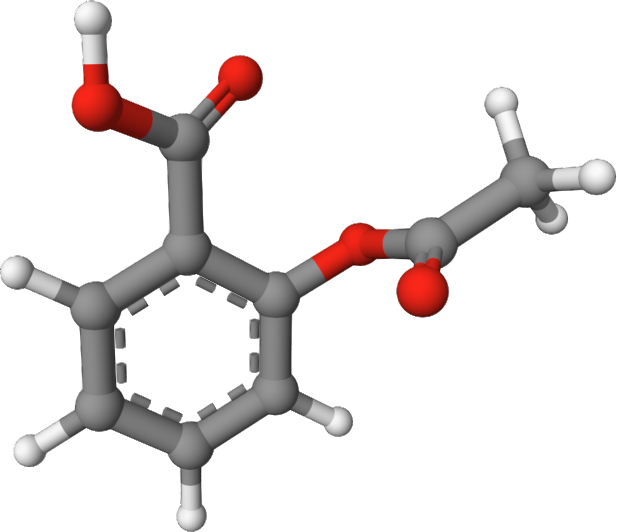
\includegraphics[width=7cm]{figures/aspirin.png}
  \end{center}
  \caption{Aspirin, a drug used to treat pain, fever, or inflammation.}
  \label{fig:aspirin}
\end{figure}

% * ✅
\subsection{Macromolecules}

Macromolecules are large molecules composed of many atoms, often thousands or even millions. They are typically formed through polymerization, where smaller subunits, called monomers, combine to form larger chain-like structures called polymers, such as proteins, nucleic acids, and carbohydrates. Macromolecules are crucial for the structure and function of cells and organisms. Their large size allows for complex interactions and the ability to carry out specialized tasks within living systems. \cite{clark2018biology,gu2009structural}

 Figure \ref{fig:hemoglobin} depicts a protein called hemoglobin, which is responsible for transporting oxygen throughout the body.

\begin{figure}[htbp]
  \begin{center}
    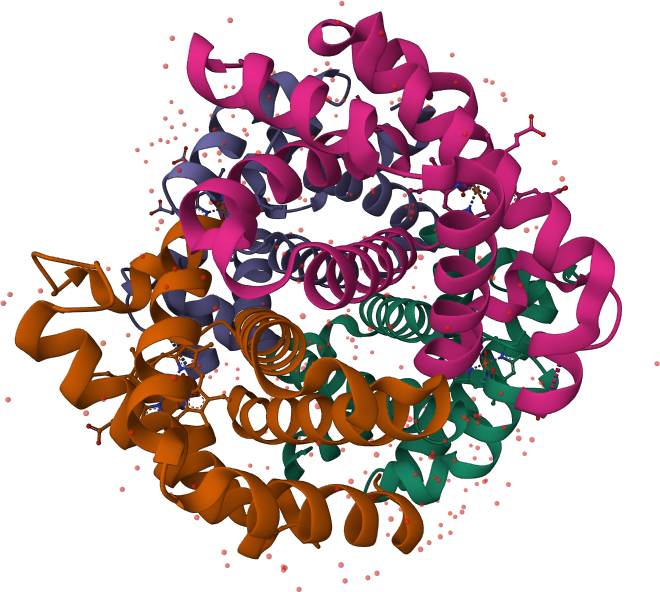
\includegraphics[width=7cm]{figures/hemoglobin.png}
  \end{center}
  \caption{Hemoglobin, a protein for transporting oxygen throughout the body.}
  \label{fig:hemoglobin}
\end{figure}

% * ✅
\subsection{Polymer structure}
\label{section:polymer_structure}

Describing macromolecules solely by their atoms and bonds becomes impractical due to the many atoms involved. Instead, macromolecules are characterized by their residues and chains.

A residue refers to a specific monomer or building block within a macromolecule. Each residue corresponds to an amino acid and nucleotide for proteins and nucleic acids, respectively. Chemical bonds link residues together to form chains. Each chain within a macromolecule is assigned a unique identifier, usually described by letters, starting with the letter A. Residues inside a chain are identified by a number, starting with the number 1. \cite{gu2009structural}

The structure of a macromolecule can be described at different levels, each providing a distinct perspective and level of abstraction. The primary structure refers to the sequence of monomers in the polymer chain. The secondary structure involves local folding patterns within the polymer chain, such as alpha helices and beta sheets in proteins. The tertiary structure encompasses the overall 3D shape of the macromolecule. Finally, the quaternary structure describes the interactions between multiple macromolecules. \cite{branden1999introduction, pdb101_hierarchical}

Figure \ref{fig:structure1} displays the ternary structure of a protein consisting of two chains, A and B. The figure focuses on chain B, which is colored to emphasize its primary structure - the sequence of its residues. Figure \ref{fig:structure2} depicts one of the residues of chain B, ARG 19, which corresponds to the 19th residue in chain B and represents the amino acid arginine.

\begin{figure}[htbp]
  \centering
  \subfigure[Residues of chain B.]{\label{fig:structure1}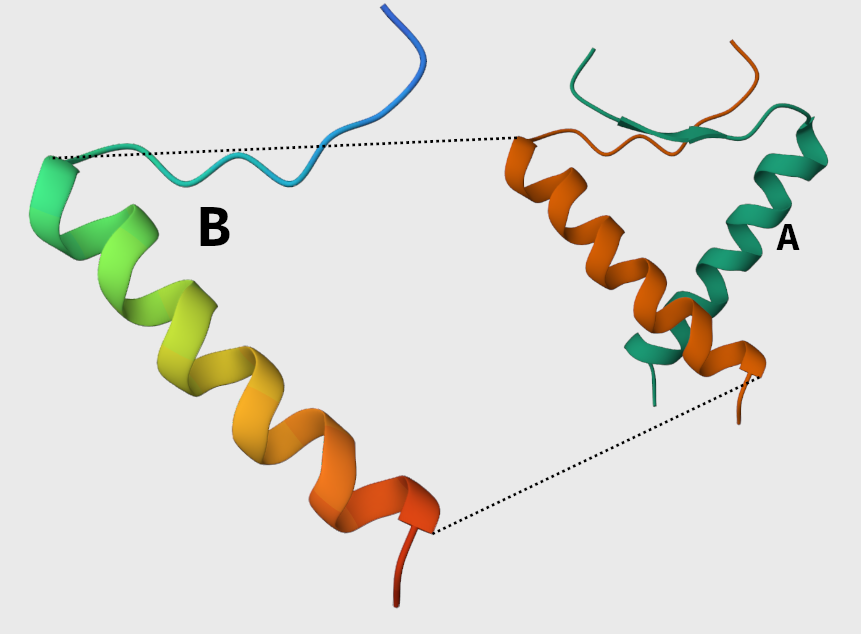
\includegraphics[height=4.5cm]{figures/structure1.png}}
  \subfigure[Atoms of residue ARG 19.]{\label{fig:structure2}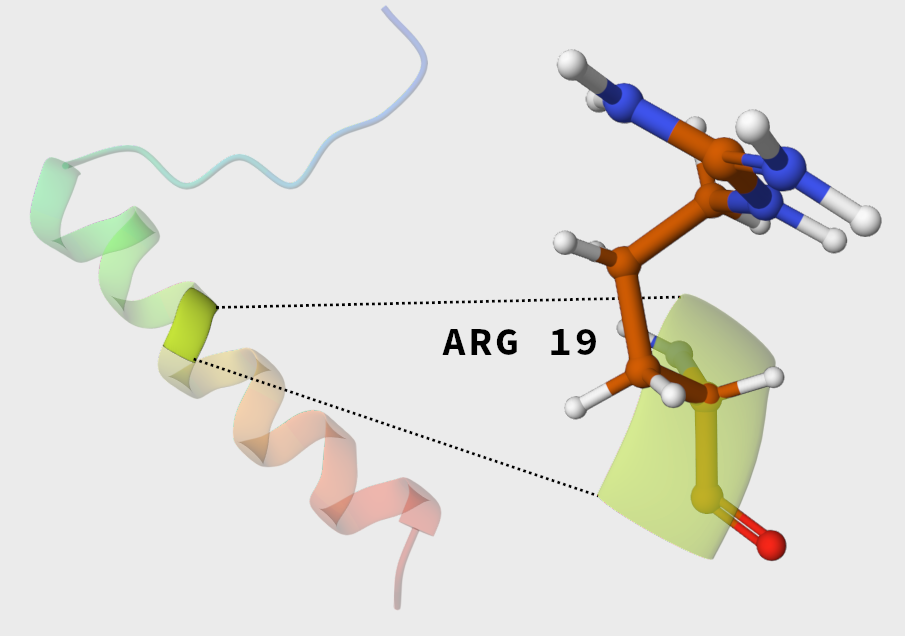
\includegraphics[height=4.5cm,]{figures/structure2.png}}
  \caption{Hierarchy of a protein structure.}
  \label{fig:structure}
\end{figure}

% * ✅
\subsection{Conformational isomers}
\label{section:alternative_conformations}

Conformational isomers, or alternative conformations, are different spatial arrangements of atoms within a molecule. \cite{conformational_isomerism} Figure \ref{fig:alternative_conformations} shows two conformational isomers of adenosine triphosphate. One conformation is colored yellow, while the other is colored blue.

\begin{figure}[htbp]
  \begin{center}
    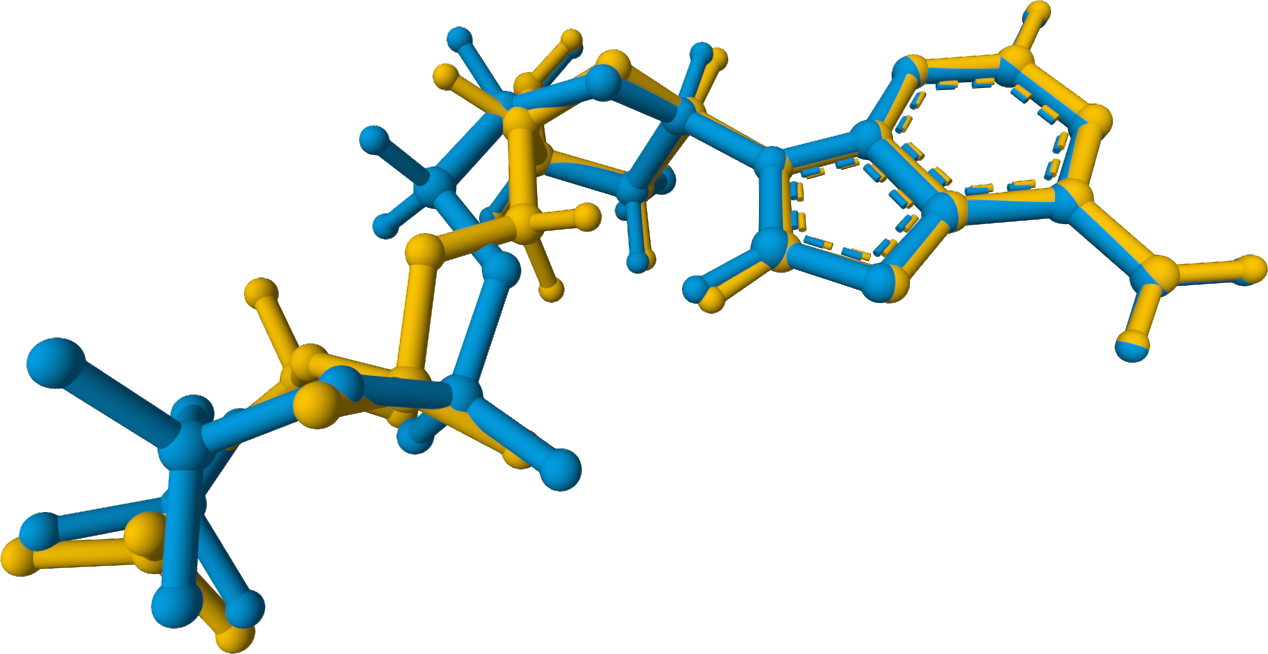
\includegraphics[width=7cm]{figures/alt_conformations.png}
  \end{center}
  \caption{Alternative conformations of ATP.}
  \label{fig:alternative_conformations}
\end{figure}


% * ✅
\section{Partial atomic charges}
\label{section:partial_atomic_charges}

When two atoms form a chemical bond, they share electrons. The electrons are not evenly shared between the two atoms due to differences in their electronegativities \footnote[1]{Electronegativity is a measure of an atom's ability to attract electrons towards itself. \cite{clark2018biology}}. Atoms with higher electronegativities attract electrons more strongly than atoms with lower electronegativities. This uneven distribution of electron density influences the physical properties of the molecule and determines how it interacts with other molecules or substances. One way of representing this uneven distribution of electron density is by assigning partial atomic charges to individual atoms within the molecule. \cite{schindler2019thesis}

Partial atomic charges are numerical values assigned to individual atoms within a molecule, representing their contribution to the distribution of electron density. Atoms with higher electronegativities have a partial negative charge (denoted as $\delta-$), while atoms with lower electronegativities have a partial positive charge (denoted as $\delta+$). \cite{racek2022thesis}

Figure \ref{fig:psilocybin} demonstrates the unequal distribution of electron density in psilocybin \cite{pubchem_psilocybine}, a psychedelic compound found in certain species of mushrooms. The figure shows the partial atomic charges colored by their values. The partial negative charges are colored red, while the partial positive charges are colored blue.

\begin{figure}[htbp]
  \begin{center}
    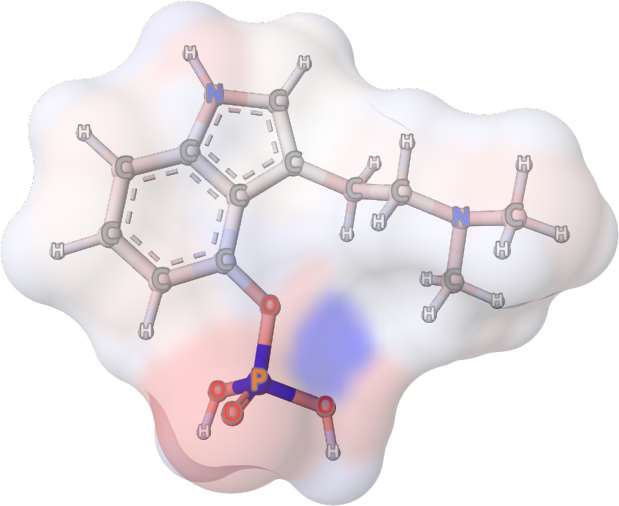
\includegraphics[width=7cm]{figures/psilocybine.png}
  \end{center}
  \caption{Partial atomic charges of psilocybin.}
  \label{fig:psilocybin}
\end{figure}

% TODO: maybe remove the citations here?

There are several applications for partial atomic charges in computational chemistry, such as molecular dynamics \cite{nejad2018insulin}, molecular docking \cite{docking}, and pharmacophore design \cite{stalke2011meaningful}. \cite{racek2022thesis,schindler2021thesis}

It is important to note that partial charges are a theoretical concept and cannot be directly measured or observed; they can only be calculated using computational methods. \cite{schindler2019thesis} 

% * ✅
\subsection{Calculation methods}
\label{section:calculating_partial_atomic_charges}

One approach to calculating partial atomic charges is by quantum mechanical methods \cite{gupta2015principles}. However, these methods are computationally expensive and require a lot of computational resources. Another approach is by empirical methods.

Empirical methods aim to produce charges comparable to those obtained through quantum mechanical methods while keeping the computational complexity manageable. Empirical methods can contain a variety of parameters. These parameters are typically derived from experimental data or quantum mechanical calculations. \cite{racek2022thesis}

There are several empirical methods for calculating partial atomic charges, such as SQE \cite{nistor2006generalization}, EEM \cite{mortier1986electronegativity}, and QEq \cite{rappe1991charge}. These methods are implemented in the ChargeFW2 \cite{racek2020acc2} program, which is used in this thesis.

% * ✅
\subsection{ChargeFW2}
\label{section:chargfw2}

ChargeFW2 is a C++ program that calculates partial atomic charges by empirical methods. The program supports 20 empirical methods, including SQE, EEM, and QEq, which were mentioned previously. It provides a command-line interface for running calculations and supports several file formats for input and output. \cite{racek2020acc2}

% * ✅
\section{Chemical file formats}
\label{section:chemical_file_formats}

Chemical file formats are used to store molecular data in a computer-readable format. There are several file formats for storing molecular data, each suited to a specific purpose.

This section explores the SDF and MOL2 file formats, commonly used for storing small molecules, and the PDB and mmCIF file formats, commonly used for storing macromolecules, such as proteins.

% * ✅
\subsection{SDF}
\label{subsection:sdf}

The Structure-Data File (SDF) is a widely used text-based chemical file format used to describe the atoms, bonds, and atomic coordinates of small molecules. It acts as a container for the MOL V2000 and V3000 file formats, allowing the storage of multiple molecules in a single file. The MOL V2000 format is a fixed-width format that can store up to 999 atoms and bonds, while the MOL V3000 format removes this limitation, enabling the storage of larger molecules \cite{mdl_ctfile,wikipedia_ctfile}.

Figure \ref{fig:sdf} depicts an SDF file containing the structure of ethanol in the MOL V2000 format. This format consists of a header section, an atom section, and a bond section. The header section contains the molecule's name, as well as the number of atoms and bonds. The atom and bond sections provide the corresponding atom and bond information, respectively \cite{belford2017anatomy}.

\begin{figure}[htbp]
  \begin{center}
    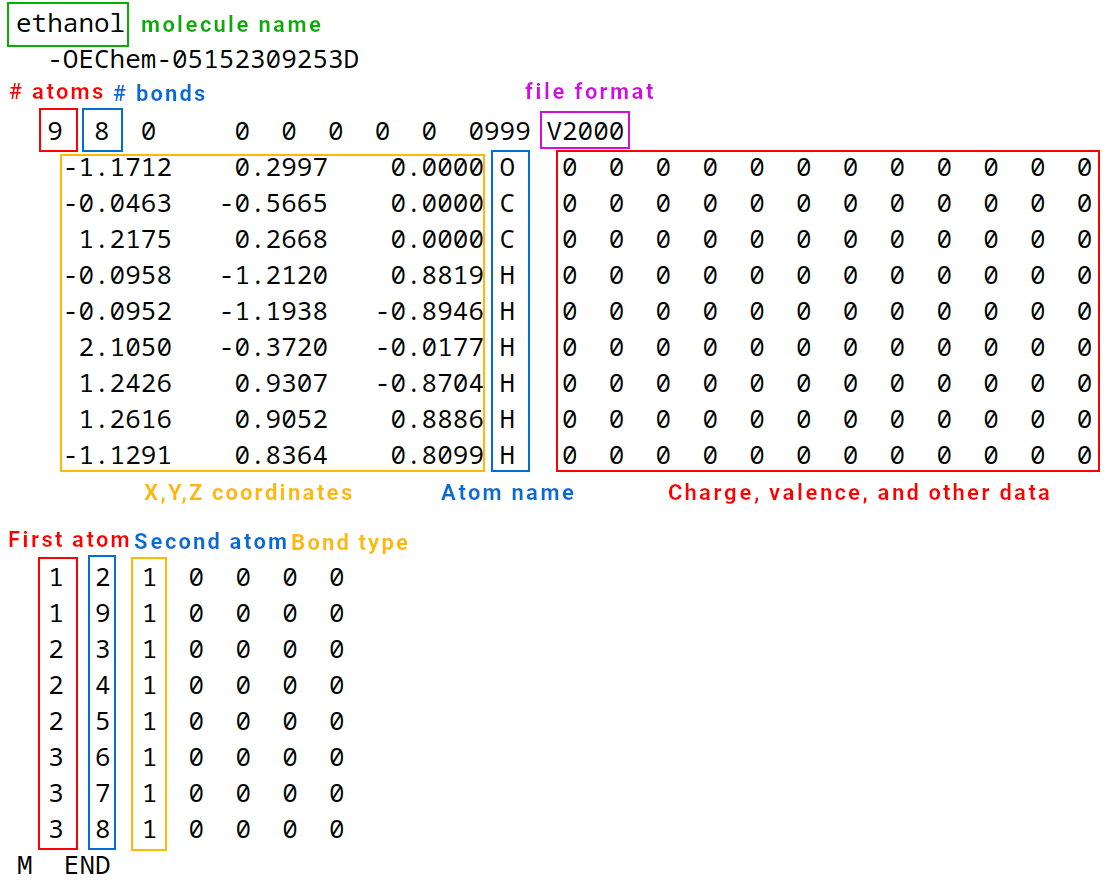
\includegraphics[width=11cm]{figures/sdf_file_format.png}
  \end{center}
  \caption{SDF file containing the structure of ethanol. \cite{belford2017anatomy}}
  \label{fig:sdf}
\end{figure}

% * ✅
\subsection{MOL2}
\label{subsection:mol2}

The Mol2 file format is another text-based format used for storing small molecular structures and their associated properties. It supports multiple conformations of a molecule and is commonly utilized in molecular modeling and cheminformatics applications. Compared to the SDF format, Mol2 provides more flexibility and additional features by supporting various record types, including custom charge data.\cite{manish}

Figure \ref{fig:mol2} illustrates the contents of an MOL2 file containing the structure of ethanol. Notice the similarity between the MOL2 and SDF formats. Both formats contain the same information about atoms and bonds. However, the MOL2 format offers greater flexibility in its structure.

\begin{figure}[htbp]
  \begin{center}
    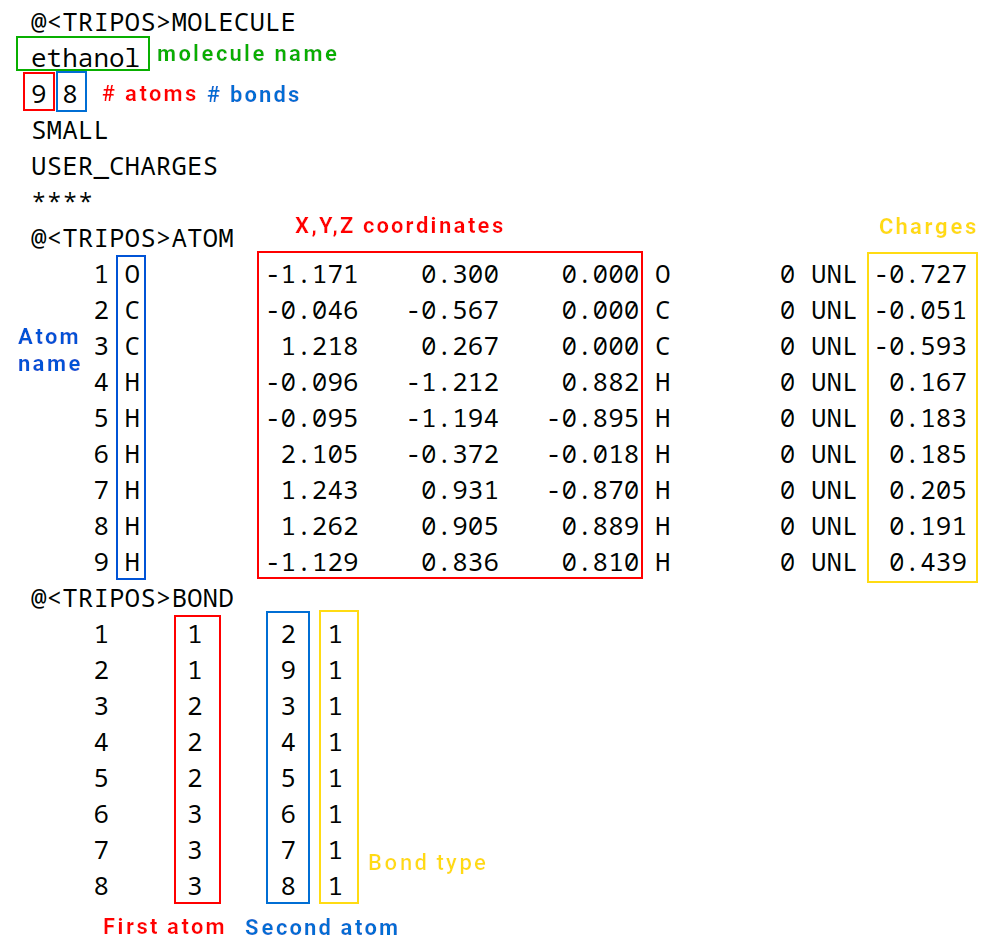
\includegraphics[width=11cm]{figures/mol2_file_format.png}
  \end{center}
  \caption{MOL2 file containing the structure of ethanol.}
  \label{fig:mol2}
\end{figure}

% * ✅
\subsection{PDB}
\label{subsection:pdb}

The Protein Data Bank (PDB) file format is widely employed for storing three-dimensional structures of proteins, nucleic acids, and other macromolecules. PDB files contain vital information such as atomic coordinates, secondary structure, and other essential details required for understanding macromolecular structures. The PDB format has found extensive use in structural biology, bioinformatics, and related fields. \cite{pdb101}

The PDB format consists of rows of records. Each record begins with a keyword identifying the record type, such as ATOM, HETATM, or CONECT. Figure \ref{fig:pdb} displays the ATOM record section of a PDB file containing the structure of a hemoglobin protein. This record section contains the atomic coordinates of the protein's atoms and other information, such as the atom's name, residue name, and residue number. \cite{chimera_pqrfile}

\begin{figure}[htbp]
  \begin{center}
    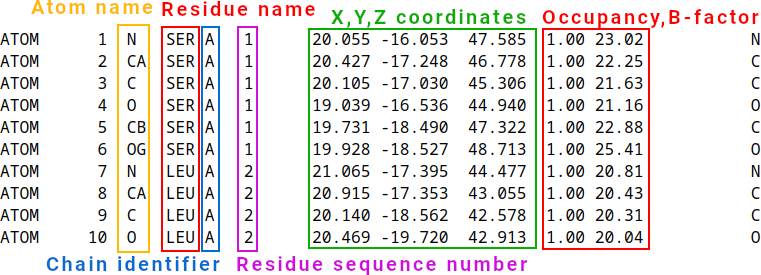
\includegraphics[width=11cm]{figures/pdb_format.png}
  \end{center}
  \caption{The ATOM record section of a PDB file containing the structure of a hemoglobin protein.}
  \label{fig:pdb}
\end{figure}

% * ✅
\subsection{PQR}
\label{subsection:pqr}

The PQR format is a non-standard variant of the PDB format that enables users to include partial atomic charges and radii parameters in the existing PDB data. It replaces the Occupancy and B-factor fields (see Figure \ref{fig:pdb}) with fields for partial atomic charges and radii. \cite{pqrfile,apbs_pqrfile} Despite the PQR format being non-standard, it is still used in some applications, such as the Atomic Charge Calculator II, for storing partial atomic charges. \cite{racek2020acc2}.

% * ✅
\subsection{mmCIF}
\label{subsection:mmcif}

The mmCIF format, also known as PDBx/mmCIF, offers an enhanced and flexible representation of macromolecular crystallography data compared to the PDB format. One of its most significant advantages is the utilization of data dictionaries, allowing users to define new data items and incorporate additional information into the file. Unlike other formats, mmCIF does not limit column width and entry count, making it more flexible and accommodating for storing large amounts of data \cite{qtpie}.

The mmCIF file format stores all data items in a relational database format. Data items are stored in separate tables. The tables are linked together with unique identifiers (pointers). Furthermore, a unique token identifies and references each data item in the file. A token comprises a category name and an attribute name separated by a dot. For example, the token \texttt{\_atom\_site.id} refers to the \texttt{id} data item in the \texttt{\_atom\_site} category. Furthermore, the mmCIF format supports two forms of storing data items: key-value and tabular. Key-value data items contain a single value, while tabular data items contain multiple values. Multi-valued data items are represented as a list of values separated by a newline character. \cite{pdb101}

Figure \ref{fig:mmcif} depicts the \texttt{\_atom\_site} category in the mmCIF file containing hemoglobin. This category is represented in tabular form, indicated by the \texttt{\_loop} token on the first row. Each row of the table corresponds to an atom in the structure. The \texttt{\_atom\_site} category contains several data items, including the following \cite{mmcif_dictionary}:

\begin{itemize}
  \item \texttt{\_atom\_site.id}: a unique identifier for each atom in the structure
  \item \texttt{\_atom\_site.label\_atom\_id}: the name of the atom (unique \\
  within the residue)
  \item \texttt{\_atom\_site.label\_comp\_id}: the name the residue containing the atom
  \item \texttt{\_atom\_site.label\_seq\_id}: the sequence number of the residue containing the atom
  \item \texttt{\_atom\_site.label\_comp\_id}: the name of the chain containing the atom
  \item \texttt{\_atom\_site.label\_alt\_id}: the alternate conformation indicator for the atom
\end{itemize}

\begin{figure}[htbp]
  \begin{center}
    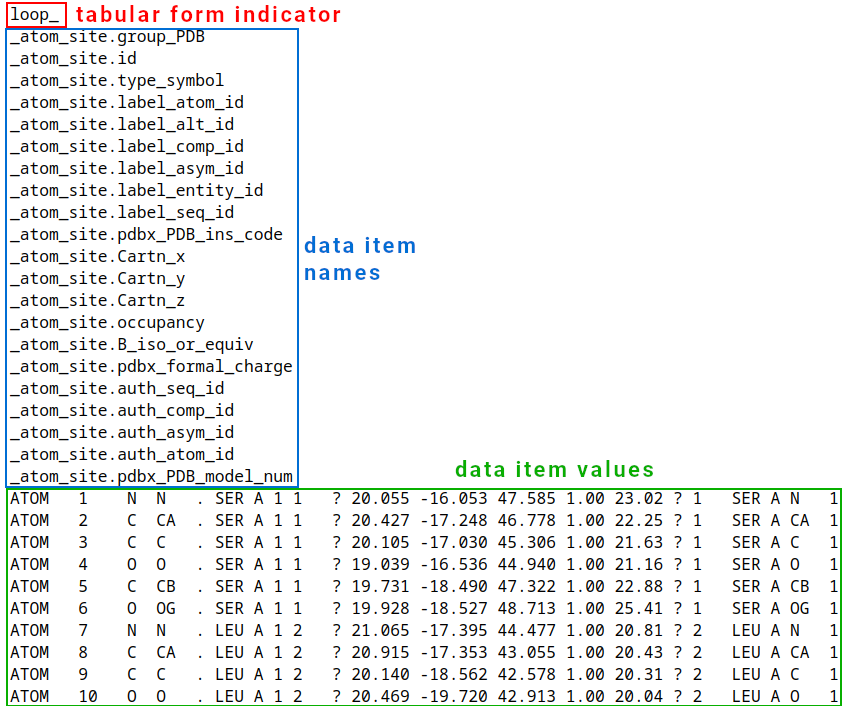
\includegraphics[width=11cm]{figures/3bj1_mmcif.png}
  \end{center}
  \caption{Tabular representation of the \texttt{\_atom\_site} data items in the mmCIF format for hemoglobin.}
  \label{fig:mmcif}
\end{figure}

\section {Color interpolation}
\label{section:color_interpolation}

% TODO: this is a bit too short, maybe add more details

% TODO: plagiarism

Color interpolation refers to the process of determining intermediate colors between two or more given colors. This is typically done by taking a weighted average of the red, green, and blue values of the interpolated colors. It is a common technique used in computer graphics to smoothly transition between colors or to generate new colors based on existing ones. \cite{zucconi2016secrets}

\newpage

% * ✅
\chapter{Visualizing molecular data}
\label{chapter:visualizing_molecular_data}

The chemical file formats discussed in Section \ref{section:chemical_file_formats} provide a convenient way of storing molecular data. However, they alone do not provide an efficient way of interpreting the data, especially for large structures. The data needs to be visualized to comprehend and extract meaningful insights from the data. \cite{gu2009structural}

This chapter explores the various types of visualizations and color schemes used to represent molecular data. It also discusses the different visualization tools available for visualizing molecular data.

\section{Types of visualizations}
\label{section:types_of_visualizations}

% TODO: plagiarism

There are several methods for representing molecular data, each serving a different purpose and providing a different level of detail. The methods most relevant to this work are the following three types: ball and stick, surface, and cartoon. The following sections describe these methods in more detail.

\subsection{Ball and stick}
\label{subsection:ball_and_stick}

The ball and stick model represents atoms as spheres and bonds as cylindrical connections between these spheres. This ball and stick model provides a simple and intuitive visualization of a molecule's atomic structure. It highlights individual atoms and their bonds, including their bond types. \cite{tsai2003introduction} However, it is not suitable for visualizing larger molecules due to the large number of atoms and bonds that would need to be displayed.

Examples of ball and stick representations are shown in Figures \ref{fig:structure2}, \ref{fig:element_symbol}, and \ref{fig:partial_charges_color_theme-bas}.

\subsection{Surface}
\label{subsection:surface}

Surface representations depict the three-dimensional shape of a molecule by displaying its solvent-accessible surface. This model provides a more accurate representation of the molecule's overall shape and size, making it especially useful for studying macromolecular interactions and the binding of small molecules.
For example, surface visualization can be used to identify potential binding sites on a protein surface, which can then be targeted by drug molecules. \ref{docking}

Examples of surface models are shown in Figures \ref{fig:psilocybin} and \ref{fig:partial_charges_color_theme-surface}.

\subsection{Cartoon}
\label{subsection:cartoon}

Cartoon representations simplify the molecular structure by focusing on the secondary structure elements of proteins and nucleic acids, such as alpha helices and beta sheets. Alpha helices are often depicted as spiral-like structures, whereas beta sheets as arrows. This type of visualization is beneficial for visualizing large macromolecular complexes, as it highlights the overall organization and topology of the molecule without the clutter of atomic details. \cite{gu2009structural,tsai2003introduction}

Figure \ref{fig:cartoon} shows an example of an alpha helix and beta sheet of a protein. Examples of cartoon representations are shown in Figures \ref{fig:hemoglobin} and \ref{fig:partial_charges_color_theme-cartoon}.

\section{Coloring of molecular visualizations}
\label{subsection:coloring_of_molecular_visualizations}

The coloring scheme used to represent the molecular structure is equally important as the visualization type. Coloring molecular structures can provide additional information and help emphasize specific molecule features and properties.

\begin{itemize}
  \item \textbf{Element symbol}: atoms are colored according to their chemical element (e.g., carbon in grey, oxygen in red, nitrogen in blue). This coloring is useful for distinguishing between different types of atoms in a molecule. See Figure \ref{fig:element_symbol} for an example.
  \item \textbf{Chain identifier}: atoms or residues are colored according to their chain identifier (e.g., chain A in blue, chain B in red). This coloring is useful for distinguishing between different chains in a macromolecular complex. See Figure \ref{fig:chain_id_coloring} for an example.
  \item \textbf{Partial atomic charge}: this coloring is explained in Section \ref{section:partial_atomic_charges}. See Figure \ref{fig:partial_charges_color_theme} for additional coloring examples.
\end{itemize}

\begin{figure}[htbp]
  \centering
  \subfigure[Example of α-helix and β-sheet representation.]{\label{fig:cartoon}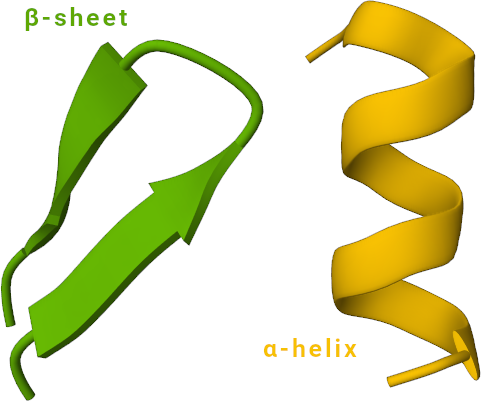
\includegraphics[height=4.5cm]{figures/cartoon.png}}
  \subfigure[Element symbol.]{\label{fig:element_symbol}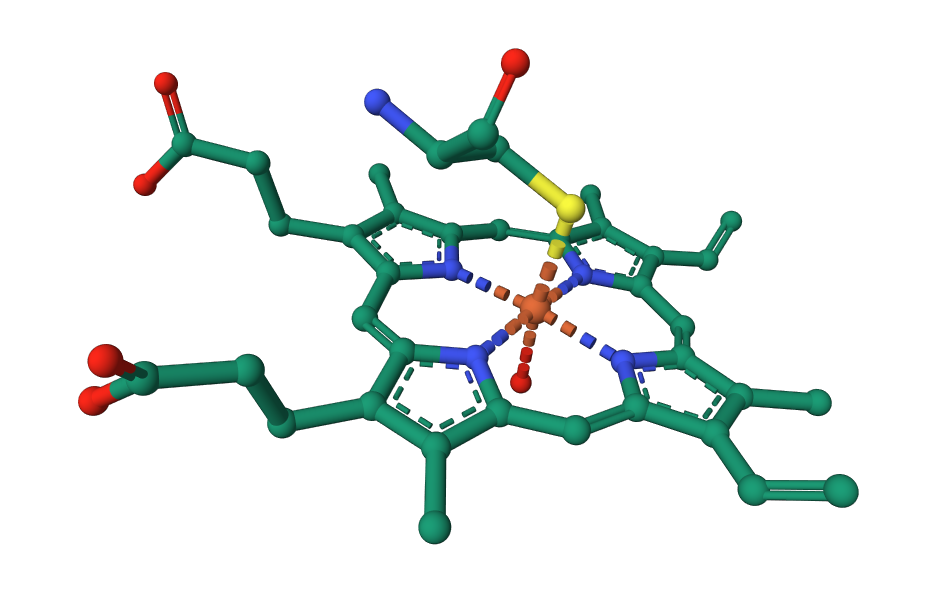
\includegraphics[height=4.5cm]{figures/ball_and_stick.png}}
  \subfigure[Chain ID.]{\label{fig:chain_id_coloring}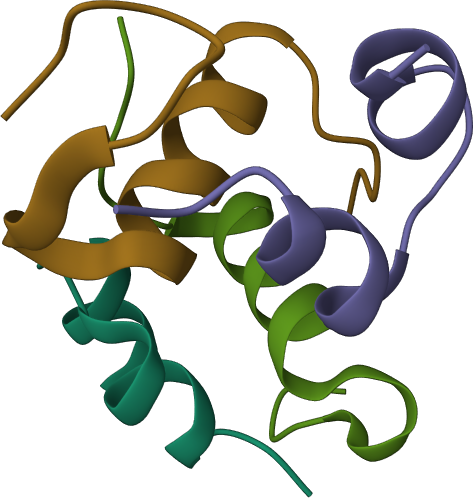
\includegraphics[height=4.5cm]{figures/chain_id_coloring.png}}
  \caption{Coloring of molecular structures by various color schemes.}
  \label{fig:coloring}
\end{figure}

\section{Visualization software}
\label{section:visualization_software}

% TODO: describe the web based \\

There are numerous software tools available for visualizing molecular data, with varying levels of complexity, customization, and features. Some of the most popular tools include MolScript \cite{kraulis1991molscript}, PyMOL \cite{delano2002pymol}, VMD \cite{humphrey1996vmd}, and ChimeraX \cite{goddard2018ucsf}. More recently, web-based visualization tools, such as NGL Viewer \cite{rose2015ngl}, LiteMol \cite{sehnal2017litemol}, and Mol* \cite{sehnal2021molstar}, have become increasingly popular due to their accessibility and ease of use.

In the following sections, we will discuss the two web-based molecular visualization tools used in this work, LiteMol and Mol*, focusing on the latter.

\subsection{Litemol}
\label{subsection:litemol}

% TODO: explain screenshot

LiteMol is an open-source tool suite for molecular data visualization. It supports various file formats and offers a user-friendly interface for creating visualizations. LiteMol provides essential visualization types, including ball and stick, surface, and cartoon representations, as well as options for customizing colors, lighting, and other display settings. The web-based nature of LiteMol makes it easily accessible and platform-independent. \cite{sehnal2017litemol}

Figure \ref{fig:litemol} shows an example of a LiteMol visualization of the 1CBS protein structure. 

\begin{figure}[htbp]
  \begin{center}
    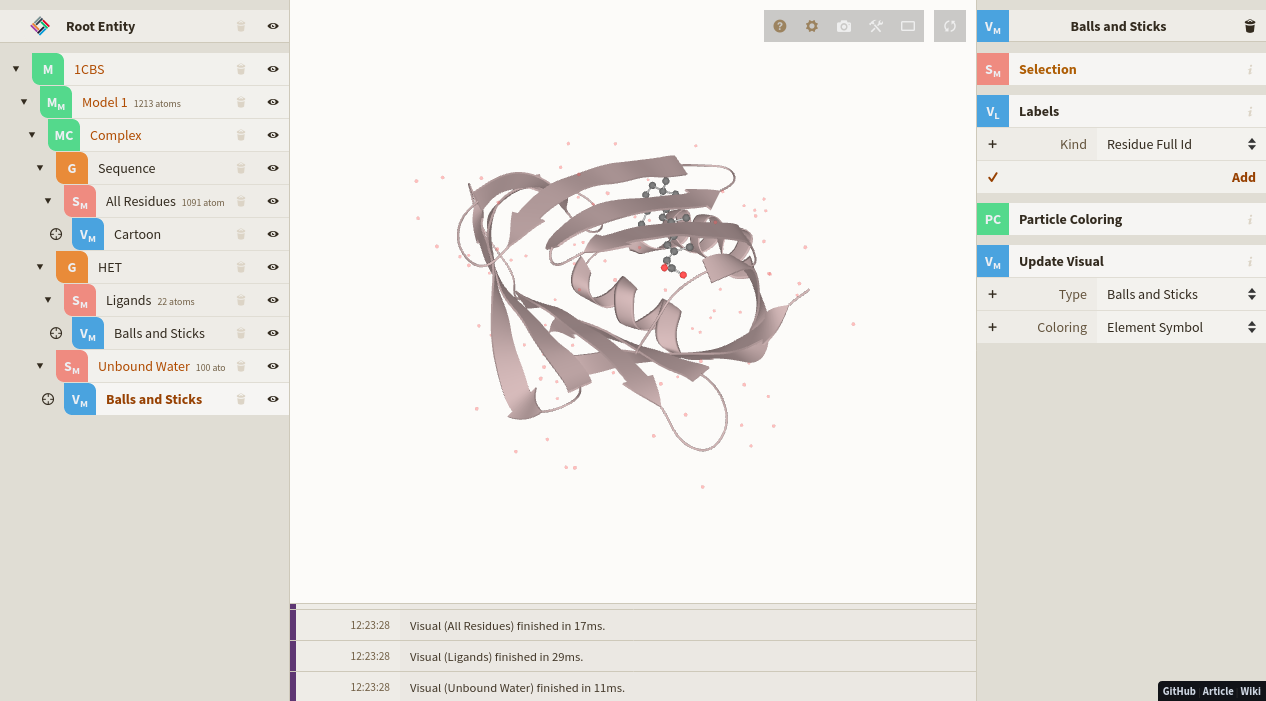
\includegraphics[width=\textwidth]{figures/litemol.png}
  \end{center}
  \caption{Litemol visualization of the 1CBS protein structure.}
  \label{fig:litemol}
\end{figure}

\subsection{Mol*}
\label{subsection:molstar}

% TODO: explain screenshot

Mol* (/'molstar/) is another web-native molecular visualization tool, developed as part of the wwPDB OneDep system for macromolecular structure deposition and validation. Mol* offers a wide range of visualization options, including advanced features such as electron density maps and validation reports. Mol* supports many file formats, including PDB, mmCIF, and PDBx/mmJSON. Like LiteMol, Mol* is platform-independent and can be accessed from any web browser. \cite{sehnal2021molstar}

Mol* emphasizes interactivity and offers various tools for manipulating and analyzing the molecular structure, such as distance and angle measurements, selection and display of specific residues, and custom coloring schemes. Additionally, Mol* provides integration with external databases and services, such as UniProt, PDBe, and RCSB PDB, enabling users to quickly access related information and resources.

The Mol* library works in a modular fashion, where each representation, color theme, and other feature is implemented as a separate provider. This modular design allows for easy customization and extension of the library. \cite{sehnal2021molstar}

\begin{figure}[htbp]
  \begin{center}
    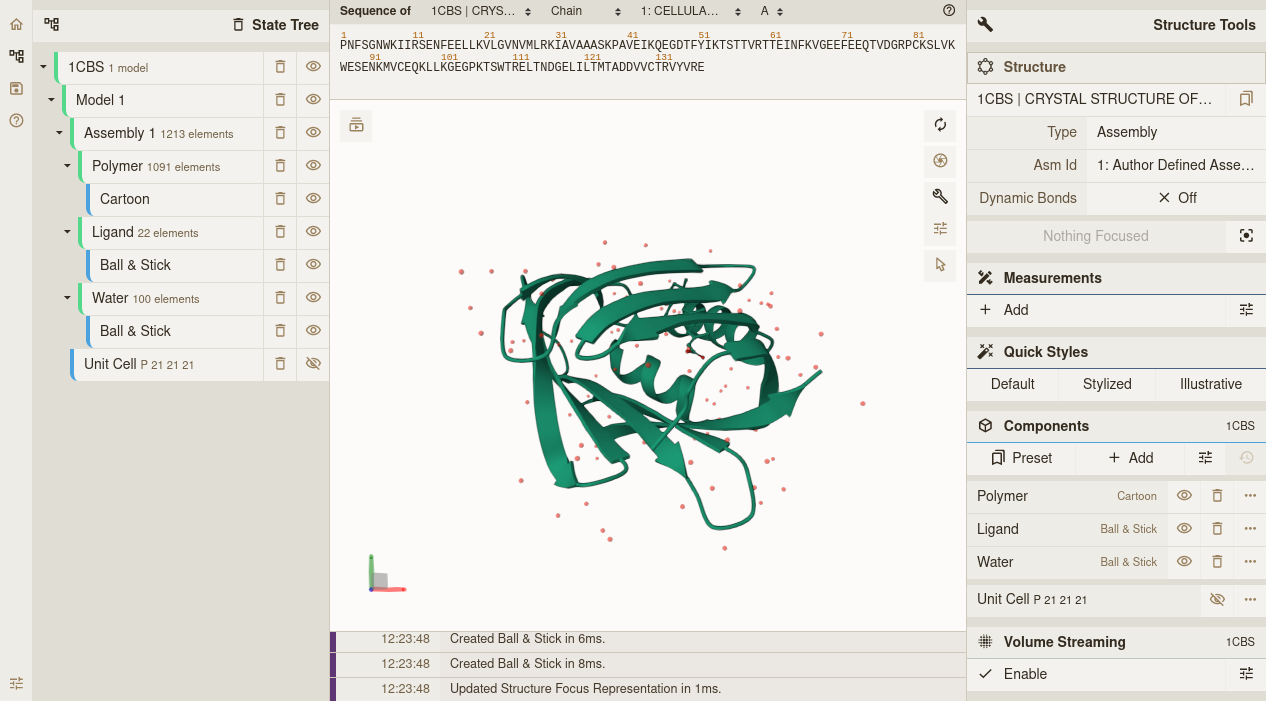
\includegraphics[width=\textwidth]{figures/molstar.png}
  \end{center}
  \caption{Mol* visualization of the 1CBS protein structure.}
  \label{fig:molstar}
\end{figure}

\subsubsection{Mol* state tree}

To store information about the molecular structure and its visualization, the Mol* library uses a state tree. The state tree is a tree data structure consisting of several layers, each of which contains information about a specific aspect of the structure. The layers are organized in a hierarchical manner, with each layer containing information about the layer below it. The state tree is a key component of the Mol* library, as it allows for easy access to the data and facilitates the implementation of various features. \cite{sehnal2021molstar}

% Figure \ref{fig:state_tree} shows the state tree of a molecular structure. The state tree consists of several layers. The top layer contains information about the molecular structure itself, such as the atoms and residues it contains. The layer below that contains information about the model, which represents a single state of the molecular structure. The layer below it contains information about the assembly, which organizes of multiple molecular components - such as chains, ligands, and water molecules - into a single structure. The layer below that contains information about the representation, which defines how the molecular structure is visualized. Finally, the bottom layer contains information about the color theme, which defines how the molecular structure is colored.

\begin{figure}[htbp]
  \begin{center}
    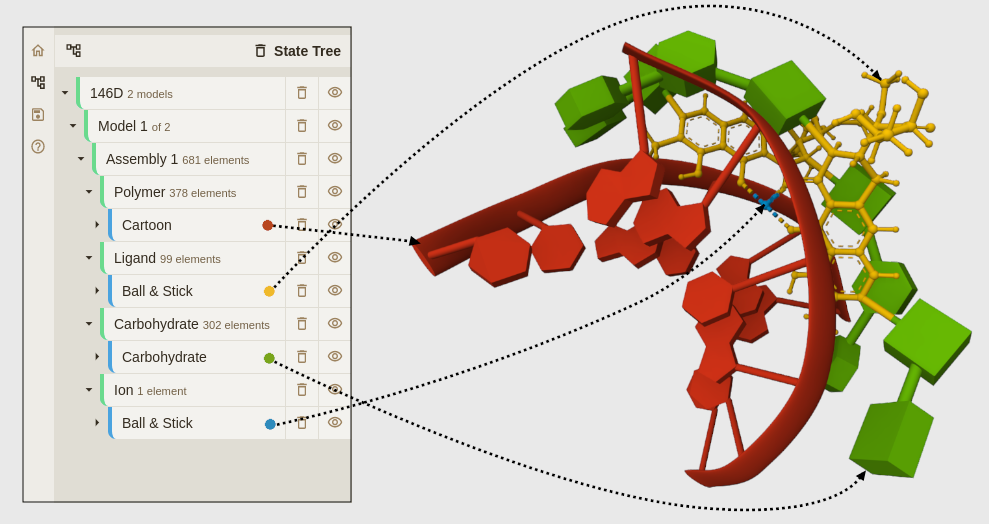
\includegraphics[width=\textwidth]{figures/state_tree.png}
  \end{center}
  \caption{Mol* state tree.}
  \label{fig:state_tree}
\end{figure}

\newpage

% * ✅
\chapter{Mol* partial charges extension}
\label{chapter:molstar_partial_charges_extension}

Visualizing partial atomic charges in molecules is an essential aspect of computational chemistry research, aiding in analyzing complex molecular structures. Mol* provides an extensive range of features for exploring molecular structures. However, the tool lacks the functionality to color and label atoms and residues based on their partial atomic charges. As mentioned in the \nameref{chap:introduction}, the Mol* viewer’s predecessor, Litemol, supported this functionality. Nevertheless, since Litemol is no longer supported, we saw the need to bring this functionality to Mol*.

This chapter describes the requirements for the extension, the custom mmCIF categories necessary for storing the partial atomic charges, and the implementation of the extension itself.

% * ✅
\section{Requirements}
\label{section:requirements}

Firstly, the Mol* extension should enable coloring atoms and residues according to their corresponding atom or residue partial atomic charges. By residue charges, it is meant the sum of the partial atomic charges of all atoms within a residue. The extension should also support the ball and stick, surface, and cartoon representations.

Secondly, it should describe the charge values of the atoms and residues.

Thirdly, the extension should allow the user to provide multiple charge sets for a single structure and to select which one to display. Finally, the extension should be seamlessly integrated into the Mol* library, facilitating access to its features and functionality.

\section{Custom mmCIF categories}
\label{section:custom_mmcif_categories}

Storing the structure and partial atomic charges in a single file was a crucial aspect of the extension. It provides a smoother process of loading the input structure file into the Mol* viewer. If the charges were stored separately, it would have been necessary to provide the charge data to Mol* by different means, e.g., through custom Mol* import controls.

For this purpose, we have chosen the mmCIF file format and designed two custom mmCIF categories, one for storing the partial charge values for each atom in the structure and another for storing metadata about the charge sets.

The mmCIF format was chosen because it is widely used in the field of structural biology and offers several advantages over other formats, as discussed in \ref{subsection:mmcif}. The custom categories allow us to store information about the partial atomic charges separately from the other structural data while still being able to access it within the same file.

The category \texttt{\_sb\_ncbr\_partial\_atomic\_charges\_meta} stores \\ metadata about the charge sets, such as the method used to calculate the charges and the type of the calculation method. The attributes of the category are listed in Table \ref{table:partial_atomic_charges_meta}.

\begin{table}[htbp]
  \centering
  \begin{tabular}{|p{0.3\linewidth} | p{0.6\linewidth}|}
    \hline
    \textbf{Attribute name} & \textbf{Description} \\
    \hline
    id & unique identifier of the charge set (e.g., '1') \\
    \hline
    type & type of the calculation method (e.g., 'empirical', 'quantum') \\
    \hline
    method & computation method used to calculate the charge set (e.g., 'EQeq', 'EEM/Racek 2016 (ccd2016\_npa)') \\
    \hline
  \end{tabular}
  \caption{Attributes of the \texttt{\_sb\_ncbr\_partial\_atomic\_charges\_meta} mmCIF category.}
  \label{table:partial_atomic_charges_meta}
\end{table}

The category \texttt{\_sb\_ncbr\_partial\_atomic\_charges} maps together the atoms of the structure and their corresponding charges. The attributes of the category are listed in Table \ref{table:partial_atomic_charges}.

\begin{table}[htbp]
  \centering
  \begin{tabular}{|p{0.3\linewidth} | p{0.6\linewidth}|}
    \hline
    \textbf{Attribute name} & \textbf{Description} \\
    \hline
    type\_id & pointer to the \texttt{id} item in the metadata category \\
    \hline
    atom\_id & pointer to the \texttt{\_atom\_site.id} item described in \ref{subsection:mmcif} \\
    \hline
    charge & partial charge value for the atom (float value) \\
    \hline
  \end{tabular}
  \caption{Attributes of the \texttt{\_sb\_ncbr\_partial\_atomic\_charges} mmCIF category.}
  \label{table:partial_atomic_charges}
\end{table}

Figure \ref{fig:mmcif_erd} provides a detailed illustration of the custom mmCIF categories and their relationships.

% TODO: check if the figure is ok

\begin{figure}
  \begin{center}
    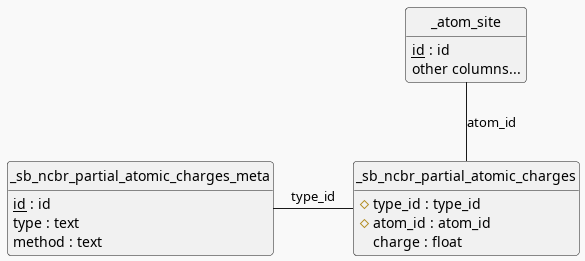
\includegraphics[width=\textwidth]{figures/mmcif_erd.png}
  \end{center}
  \caption{Diagram of the relationship of the custom mmCIF categories for storing partial atomic charges.}
  \label{fig:mmcif_erd}
\end{figure}

\section{Implementation}
\label{section:implementation}

This section will detail the implementation of the extension. The extension consists of multiple providers. Each provider serves a distinct functionality, such as supplying the partial charge data and coloring the structural elements based on their charges. The providers will be described in detail in the following subsections.

The extension was created using TypeScript, a superset of JavaScript that adds static typing and other features to the language. The Mol* library is also written in TypeScript, so the extension was written in the same language to ensure compatibility.

\subsection{Property provider}
\label{subsection:property_provider}

In order to retrieve the charges from the mmCIF file, it is necessary to parse the file. This is done by the Mol* library, which parses the mmCIF file and provides the parsed mmCIF file data in the form of a \texttt{MmcifFormat} object. The purpose of this provider is to process the charge data from this object and supply the charge data to the rest of the extension providers through a custom property. The interface of this property is depicted in Figure \ref{figure:charge_data_structure}.

The atom charges are stored in the \texttt{typeIdToAtomIdToCharge} map. The map is indexed by the charge set (typeId) and the atom id. The atom id is a pointer to the atom\_site.id. item in the mmCIF file. The atom charges are retrieved from the mmCIF file by iterating over the atom\_site.id category and retrieving the charge values for each atom. The charge values are then stored in the \texttt{typeIdToAtomIdToCharge} map.

The residue charges are calculated by summing the charges of the atoms that make up the residue. The residue charge is then stored in the \texttt{typeIdToResidueIdToCharge} map.

The maximum absolute charge values of the atoms and residues are calculated and stored in the \texttt{maxAbsoluteAtomCharges} and \\
\texttt{maxAbsoluteResidueCharges} maps. These maps are used in the color theme provider to normalize the charges to the range of 0 to 1. Additionally, the maximum absolute charge values are used to calculate the color interpolations in the color theme provider. Furthermore, the maximum absolute charge of both atoms and residues is calculated and stored in the \texttt{maxAbsoluteChargesAll} map.

Lastly, the method name used to calculate the charges of a given charge set is stored in the \texttt{typeIdToMethod} map. This map is used to display the method name in the UIs.

\begin{figure}[htbp]
  \begin{center}
    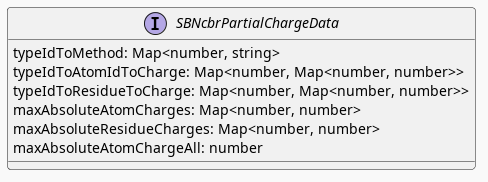
\includegraphics[width=\textwidth]{out/figures/uml/interface/custom model property interface.png}
  \end{center}
  \caption{Interface of the custom model property for storing partial atomic charges.}
  \label{fig:property_provider_interface}
\end{figure}


\begin{figure}[htbp]
  \caption{Interface of the custom model property for storing partial atomic charges.}
  \label{fig:custom_model_property}
  \definecolor{LightGray}{gray}{0.95}
  \begin{minted}[
  frame=lines,
  framesep=2mm,
  baselinestretch=1.2,
  bgcolor=LightGray,
  fontsize=\footnotesize,
  % linenos
  ]{Typescript}
    type TypeId = number;
    type IdToCharge = Map<number, number>;
    export interface SBNcbrPartialChargeData {
        typeIdToMethod: Map<TypeId, string>;
        typeIdToAtomIdToCharge: Map<TypeId, IdToCharge>;
        typeIdToResidueToCharge: Map<TypeId, IdToCharge>;
        maxAbsoluteAtomCharges: IdToCharge;
        maxAbsoluteResidueCharges: IdToCharge;
        maxAbsoluteAtomChargeAll: number;
        params: PartialChargesPropertyParams;
    }
  \end{minted}
\end{figure}

\subsection{Color theme provider}
\label{subsection:color_theme_provider}

% TODO: mention the color parameters \\

This provider serves as the central component of the extension, with its primary function being to assign colors to atoms and residues based on their charges. It achieves this by using the ColorTheme API provided by Mol*. The ColorTheme API is a mechanism for assigning colors to structural elements of a molecule. These structural elements can be atoms, residues, bonds, and so on. The API is based on the concept of a ColorTheme object, which is a collection of color assignments for structural elements. The ColorTheme object is then used by the Mol* library to color the structural elements of the molecule.

For the purposes of this extension, it was necessary to color two structural elements - atoms and residues. For both of these structural elements the charges were retrieved from the provider described in the previous section \ref{subsection:charges_provider}, which provided charges for atoms and residues.

To establish the color for a given charge, two color interpolations are employed: one for negative charges and another for positive charges. Atoms with positive charges receive a color from a white-to-blue color interpolation, while atoms with negative charges are assigned a color from a white-to-red color interpolation. These color interpolations are highlighted in Figure \ref{fig:color_gradients}. 

\begin{figure}[htbp]
  \begin{center}
    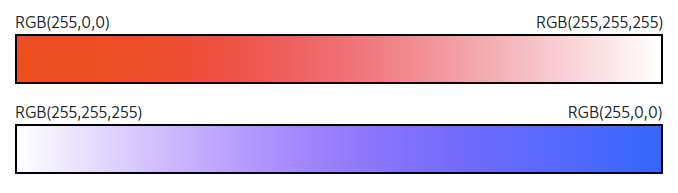
\includegraphics[width=10cm]{figures/color_gradients.png}
  \end{center}
  \caption{Color gradients representing the possible colors for positive and negative charges.}
  \label{fig:color_gradients}
\end{figure}

\begin{figure}[htbp]
  \centering
  \subfigure[Ball and stick]{\label{fig:partial_charges_color_theme-bas}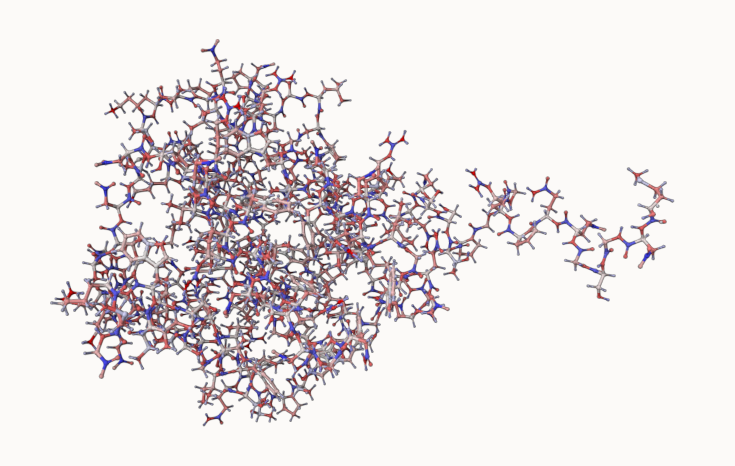
\includegraphics[width=0.45\textwidth]{figures/1F16-bas.png}}
  \subfigure[Surface]{\label{fig:partial_charges_color_theme-surface}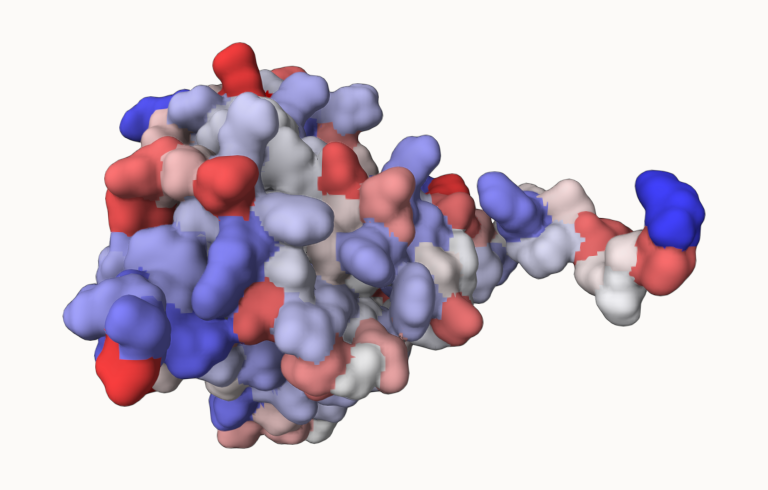
\includegraphics[width=0.45\textwidth]{figures/1F16-surface.png}}
  \subfigure[Cartoon]{\label{fig:partial_charges_color_theme-cartoon}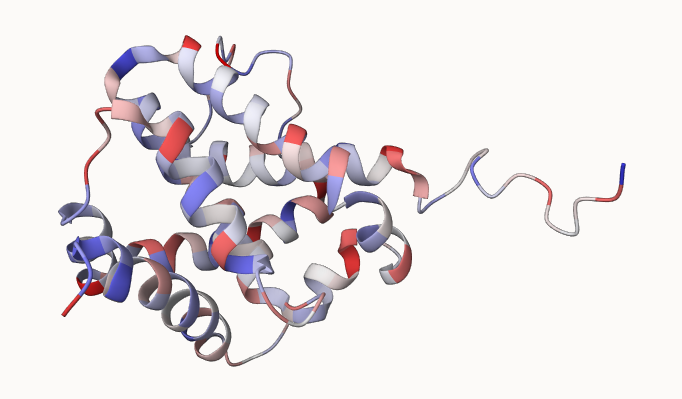
\includegraphics[width=0.45\textwidth]{figures/1F16-cartoon.png}}
  \caption{Partial charges color theme for different visualization types.}
  \label{fig:partial_charges_color_theme}
\end{figure}

\subsection{Label provider}
\label{subsection:label_provider}

% TODO: cite the Mol* documentation where the Loci object is described \\

Having colored the structural elements, it was also necessary to create a label provider, which would assign labels that describe the charge of the structural element. In order to determine which element is highlighted, Mol* uses the object Loci. A Loci object is utilized for general selections and highlights. Consequently, it is essential to first extract the location from the Loci object in order to obtain the atom ID. The charge is acquired from the property provider, and the label is an HTML string that conveys the charge of the atom or residue. An example of the label can be seen in in the right-hand corner in figure \ref{}.

\subsection{Controls}
\label{subsection:controls}

The controls are implemented automatically by the Mol* library based on the parameters of the providers. The user has access to controls of the charge set and the color theme. The charge set controls allow the user to select the charge set to display. The color theme controls allow the user to specify the following parameters:

\begin{itemize}
  \item \textbf{Charge Range}: Sets the range of the color interpolation
  \item \textbf{Use Range}: Toggles whether the range of the color interpolation is automatically calculated or manually specified.
  \item \textbf{Charge Type}: Selects whether to display the partial atomic charges or the partial residue charges.
\end{itemize}

The controls are depicted in Figure \ref{fig:controls-charge-set}.

\begin{figure}[htbp]
  \centering
  \subfigure[Charge set controls]{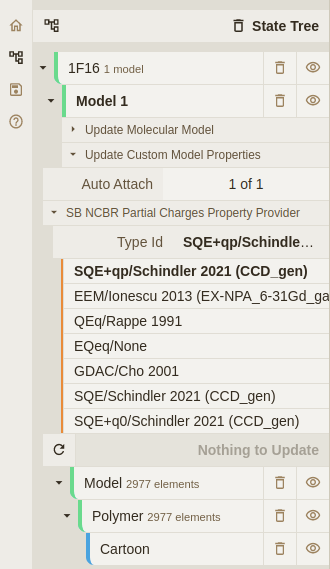
\includegraphics[width=0.49\textwidth]{figures/controls1.png}}
  \subfigure[Color theme controls]{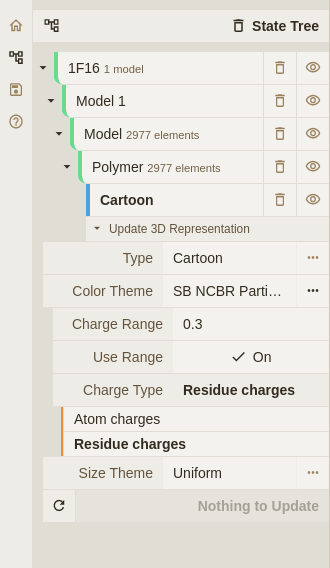
\includegraphics[width=0.49\textwidth]{figures/controls2.png}}
  \caption{Extension controls.}
  \label{fig:controls-charge-set}
\end{figure}

\section{Mol* viewer plugin}
\label{section:molstar_viewer_plugin}

In addition to the partial charges extension for the Mol* library, it was necessary to create a custom Mol* viewer plugin. By using a plugin, it is possible to create custom behavior, which is not provided by the standard Mol* viewer.

\subsection{Technologies used during development}

The plugin was developed using Vite. Vite is a build tool that was created to address some of the problems faced by developers when building large applications with traditional build tools such as Webpack. One of the main advantages of Vite is that it provides a fast development server. The speed of the development server is achieved by pre-bundling the static project dependencies with esbuild, a modern bundler written in Go, and serving the project source code with native ES module imports. \cite{vite}

The plugin is written in Typescript and uses the Mol* library. The plugin is bundled using Rollup \cite{rollup}, a module bundler for Javascript, and published to NPM, a package manager for Javascript applications. \cite{npm}

\subsection{Structure of the plugin}

The plugin is designed as a Typescript class. The structure of the class is depicted in Figure \ref{fig:plugin_structure}. It contains a method to create the plugin and another to load a structure file. Furthermore, it includes four attributes, each an object with methods that act as an interface for managing the plugin:

\begin{itemize}
  \item \textit{Charges} - provides functions for setting the charge set and retrieving information about the charge sets.
  \item \textit{Color} - provides functions for setting the color theme.
  \item \textit{Type} - provides functions for setting the visualization type.
  \item \textit{Behavior} - provides a function for focusing on a specific atom.
\end{itemize}

\begin{figure}[htbp]
  \begin{center}
    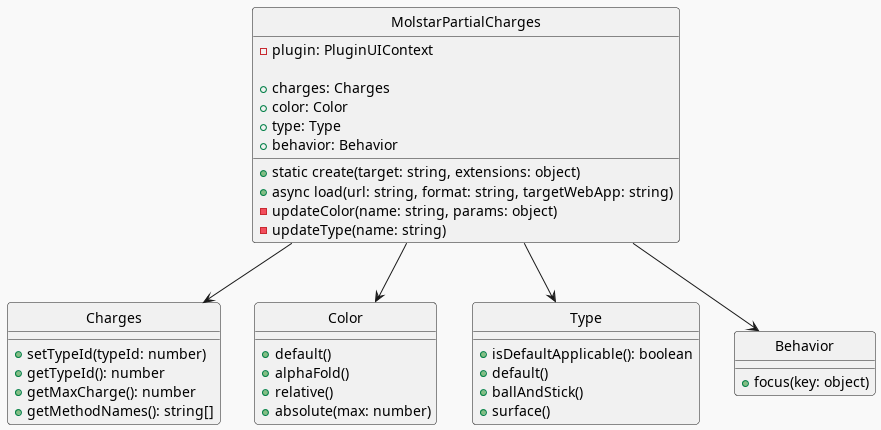
\includegraphics[width=\textwidth]{out/figures/uml/viewer/viewer.png}
  \end{center}
  \caption{Diagram of the custom Mol* viewer class.}
  \label{fig:plugin_structure}
\end{figure}

The \textit{Color} and \textit{Type} attributes set the color theme and visualization type through the private methods \textit{updateColor} and \textit{updateType}. These methods change the color theme and visualization type by iterating over the Mol* state tree and updating the representation nodes.

The focus functionality, implemented by the \textit{Behavior} attribute, is achieved by first selecting the desired atom using a query language. Mol* supports multiple query languages: MolScript, PyMOL, VMD, and Jmol. The query language used in this plugin is MolScript. The query language is used to uniquely identify and select the atom by the following attributes of the mmCIF category \textit{atom\_site}:

\begin{itemize}
  \item \textit{labelCompId} - identifier for the chain containing the residue with the atom.
  \item \textit{labelSeqId} - sequence number of the residue containing the atom.
  \item \textit{labelAtomId} - identifier for the atom in the residue.
\end{itemize}

The MolScript query selection is depicted in Figure \ref{fig:focus}. Once the atom is selected, the selection is highlighted and focused on with methods provided by the Mol* library.

\begin{figure}[htbp]
  \definecolor{LightGray}{gray}{0.95}
  \begin{minted}[
  frame=lines,
  framesep=2mm,
  baselinestretch=1.2,
  bgcolor=LightGray,
  fontsize=\footnotesize,
  % linenos
  ]{Typescript}
  const selection = Script.getStructureSelection(
    (Q) =>
        Q.struct.generator.atomGroups({
            'atom-test': Q.core.logic.and([
                Q.core.rel.eq([Q.struct.atomProperty.macromolecular.
                label_comp_id(), labelCompId]),
                Q.core.rel.eq([Q.struct.atomProperty.macromolecular.
                label_seq_id(), labelSeqId]),
                Q.core.rel.eq([Q.struct.atomProperty.macromolecular.
                label_atom_id(), labelAtomId]),
            ]),
        }),
    data
);
\end{minted}
\caption{MolScript query for selecting an atom.}
\label{fig:focus}
\end{figure}

\newpage

% * ✅
\chapter{Atomic Charge Calculator II}
\label{chapter:atomic_charge_calculator_ii}

Atomic Charge Calculator II (ACC~II) is a web application for calculating partial atomic charges for structure files. The application is built using Flask for the backend and Javascript with Bootstrap for the frontend. The core of the ACC~II application is the ChargeFW2 program, which is used to calculate the partial atomic charges. For visualizing the calculation results, the application uses the Litemol viewer. \cite{racek2020acc2} 

However, since the Litemol viewer is no longer supported, it was necessary to replace it with its modern counterpart, Mol*. This chapter describes the incorporation of the Mol* viewer into the ACC~II application. We first discuss the modifications to the ChargeFW2 program, then explain the changes made to the ACC~II application's backend and frontend to support calculations of multiple charge sets, and lastly, we describe the integration of the Mol* viewer into the ACC~II application.

% * ✅
\section{Extension of ChargeFW2}
\label{section:chargefw2_extension}

As described in Section \ref{section:chargfw2}, ChargeFW2 is a C++ program for computing partial atomic charges. The program supports the following input file formats: SDF, MOL2, PDB, and mmCIF, all of which are described in Section \ref{section:chemical_file_formats}.

The program parses the necessary atom and bond data for each molecule in the input file and stores it in a \texttt{Molecule} object. These objects are stored in a \texttt{MoleculeSet} object over which the program then iterates and calculates the partial atomic charges for each molecule.

The program outputs the charge results in multiple file formats. The following Table \ref{table:chargefw2_output_formats} lists the output file formats generated by ChargeFW2 for the corresponding input file formats.

\begin{table}[htbp]
  \centering
  \begin{tabular}{|l|l|}
    \hline
    \textbf{Input format} & \textbf{Output formats} \\
    \hline
    SDF, MOL2 & TXT, MOL2 \\
    \hline
    PDB & TXT, PQR \\
    \hline
    mmCIF & TXT, PQR, mmCIF \\
    \hline
  \end{tabular}
  \caption{ChargeFW2 output file formats.}
  \label{table:chargefw2_output_formats}
\end{table}

As seen in Table \ref{table:chargefw2_output_formats}, ChargeFW2 already outputs a mmCIF file for a corresponding mmCIF input file. The format of this output mmCIF file stores the partial atomic charges in a custom \\
\texttt{\_atom\_site.fw2\_charge} item. However, this format is incompatible with the Mol* viewer, which expects the partial atomic charges to be stored in the custom mmCIF categories described in Section \ref{section:custom_mmcif_categories}. Therefore, modifying the ChargeFW2 output was necessary.

The following subsections describe in detail how ChargeFW2 was modified to produce the custom mmCIF file format for all the input files, regardless of the format.

% * ✅
\subsection{mmCIF}

For mmCIF input files, the program simply appends the custom categories to the input file. The program uses the GEMMI library \cite{wojdyr2022gemmi} to parse the input mmCIF file into a \texttt{Block} object, which provides access to all mmCIF categories in the file. Before appending the charge categories, the program first removes alternative conformations from the \texttt{Block} object. Removing alternative conformations is necessary because the custom Mol* viewer plugin does not support alternative conformations with the partial atomic charge coloring. The program then appends the custom charge categories to the \texttt{Block} object and writes the \texttt{Block} object to the output mmCIF file.

% * ✅
\subsection{PDB}

% TODO: explain why the chem_comp category is removed

The PDB input files are first converted to mmCIF format using the GEMMI library. The PDB file is first parsed into a \texttt{Structure} object, then converted into a \texttt{Block} object. After converting the PDB file to mmCIF, it was necessary to remove the \texttt{\_chem\_comp} category from the \texttt{Block} object. GEMMI generates this category by default. However, it is unnecessary for the Mol* viewer, and its presence causes the viewer to visualize the structure incorrectly. The program then proceeds the same way as for the mmCIF input files.

% * ✅
\subsection{SDF and MOL2}

SDF and MOL2 input files are converted to mmCIF format using the atom and bond data stored in the \texttt{Molecule}. The program first creates a \texttt{Block} object, which it populates with the \texttt{\_atom\_site} category using the atom data. Secondly, it adds the \texttt{\_chem\_comp\_bond} category using the bond data. The latter category describes the bonds between the atoms and is necessary for the Mol* viewer to visualize the bond orders correctly. The program then proceeds the same way as for the mmCIF input files.

% * ✅
\subsection*{Result}

The ChargeFW2 produces a mmCIF file for each calculation, which is compatible with the Mol* viewer. This extension unifies the output file formats and enables sending just one file to the Mol* viewer on the frontend. Table \ref{table:new_chargefw2_output_formats} lists the updated output file formats generated by ChargeFW2 for the corresponding input file formats.

\begin{table}[htbp]
  \centering
  \begin{tabular}{|l|l|}
    \hline
    \textbf{Input format} & \textbf{Output formats} \\
    \hline
    SDF, MOL2 & TXT, mmCIF, MOL2 \\
    \hline
    PDB, mmCIF & TXT, mmCIF, PQR \\
    \hline
  \end{tabular}
  \caption{Updated ChargeFW2 output file formats.}
  \label{table:new_chargefw2_output_formats}
\end{table}

% * ✅
\section{Multicharge support}
\label{section:multicharge_support}

The ACC~II application allows the user to select the method and parameters that will be used to calculate the partial atomic charges for the user's input file. Once the user confirms their selection, the application sends it to the backend, which runs the ChargeFW2 program with the chosen method and parameters. The application then displays the results of the calculation to the user.

However, the application only supports one calculation per request and does not support the visualization of multiple charge sets. This limitation was previously caused by the Litemol viewer, which only supported one charge set per structure. Since the Mol* viewer supports multiple charge sets, the ACC~II application was also modified to support multiple charge sets.

The following subsections describe the necessary changes made to the ACC~II application to facilitate multiple calculations per request and the visualization of multiple charge sets.

% * ✅
\subsection{Frontend changes}

As explained in the previous section, the ACC~II application limits users to select only one combination of methods and parameters. This limitation was addressed by introducing new controls to the calculation setup.

Figure \ref{fig:new_setup} shows the updated setup page for the ACC~II application. The page now contains a list of calculations, each representing a combination of methods and parameters. The list is initially empty, and the user can add a new calculation to the list by selecting the desired method and parameters from the drop-down menus and clicking the \textit{Add to calculation} button. The user can also remove any calculation from the list by clicking the cross button next to the calculation name.

Once the user clicks the \textit{Compute} button, the list of calculations is sent to the backend, where it is used to generate the desired charge sets for the user's input file.

\begin{figure}[htbp]
  \begin{center}
    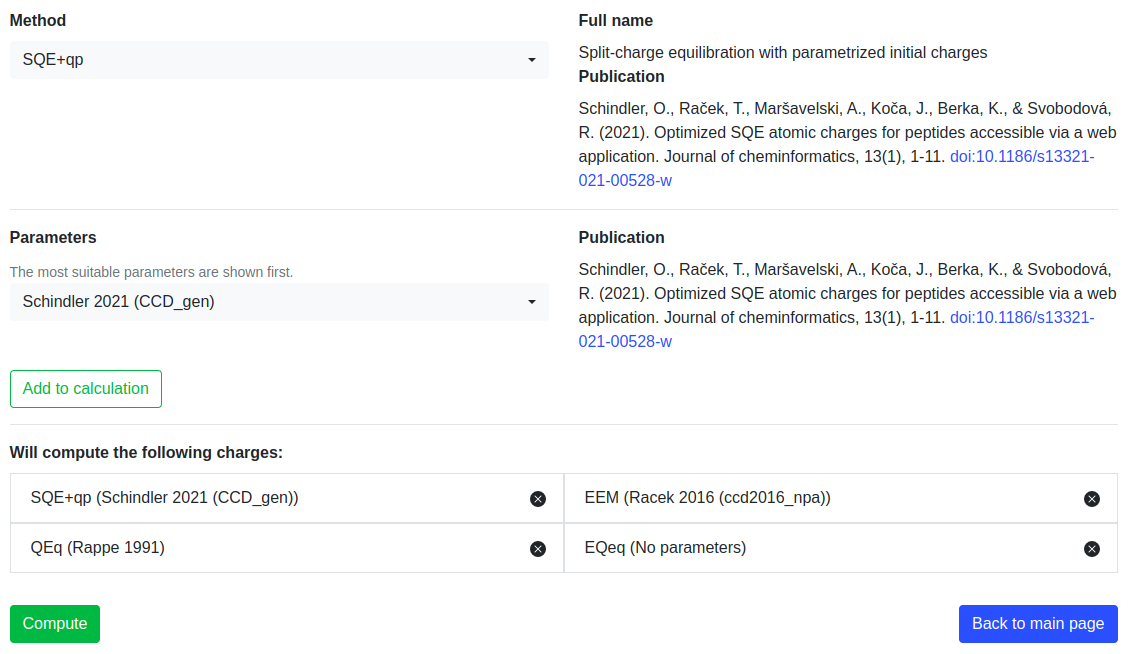
\includegraphics[width=\textwidth]{figures/new_setup.png}
  \end{center}
  \caption{Updated setup page for the ACC~II application.}
  \label{fig:new_setup}
\end{figure}

% * ✅
\subsection{Backend changes}

The Flask backend of the ACC~II application was modified to support multiple charge calculations per request. The backend now receives a list of calculations from the frontend, which it uses to generate the desired charge sets for the user's input file. It does this by running the ChargeFW2 program for each calculation in the list and generating the output file formats described in Table \ref{table:new_chargefw2_output_formats}. The backend then parses the charge values from the output TXT files and stores them in a dictionary, creating a mapping between the charge set name and the charge values.

After all of the calculations are completed, the dictionary is used to generate a single mmCIF file. Firstly, the backend parses one of the output mmCIF files generated by ChargeFW2 into a \texttt{Block} object using the GEMMI library. The backend then iterates over the dictionary and appends the charge values to the \texttt{Block} object under the custom charge categories described in Section \ref{section:custom_mmcif_categories}. Lastly, the backend writes the \texttt{Block} object to a new mmCIF file. This mmCIF file is then sent to the frontend, where it is loaded into the Mol* viewer.

% * ✅
\section{Mol* viewer integration}
\label{section:viewer_integration}

Figure \ref{fig:result_page} shows the result page for the ACC~II application with the incorporated Mol* viewer. The result page initializes the custom viewer plugin and loads the mmCIF file generated by the backend. The loaded structure can then be visualized as a ball and stick model, a surface model, or, if applicable, a cartoon model. The page also provides controls for coloring the structure by partial atomic charges or by the element symbol of each atom. The user can also set the maximum charge value, which will be used for the partial atomic charge coloring.

The result page also contains two dropdown menus. The structure dropdown menu contains all the structures the user provides in their input file. The charge set dropdown menu contains all the charge sets generated by the backend according to the user's selection on the setup page.

\begin{figure}[htbp]
  \begin{center}
    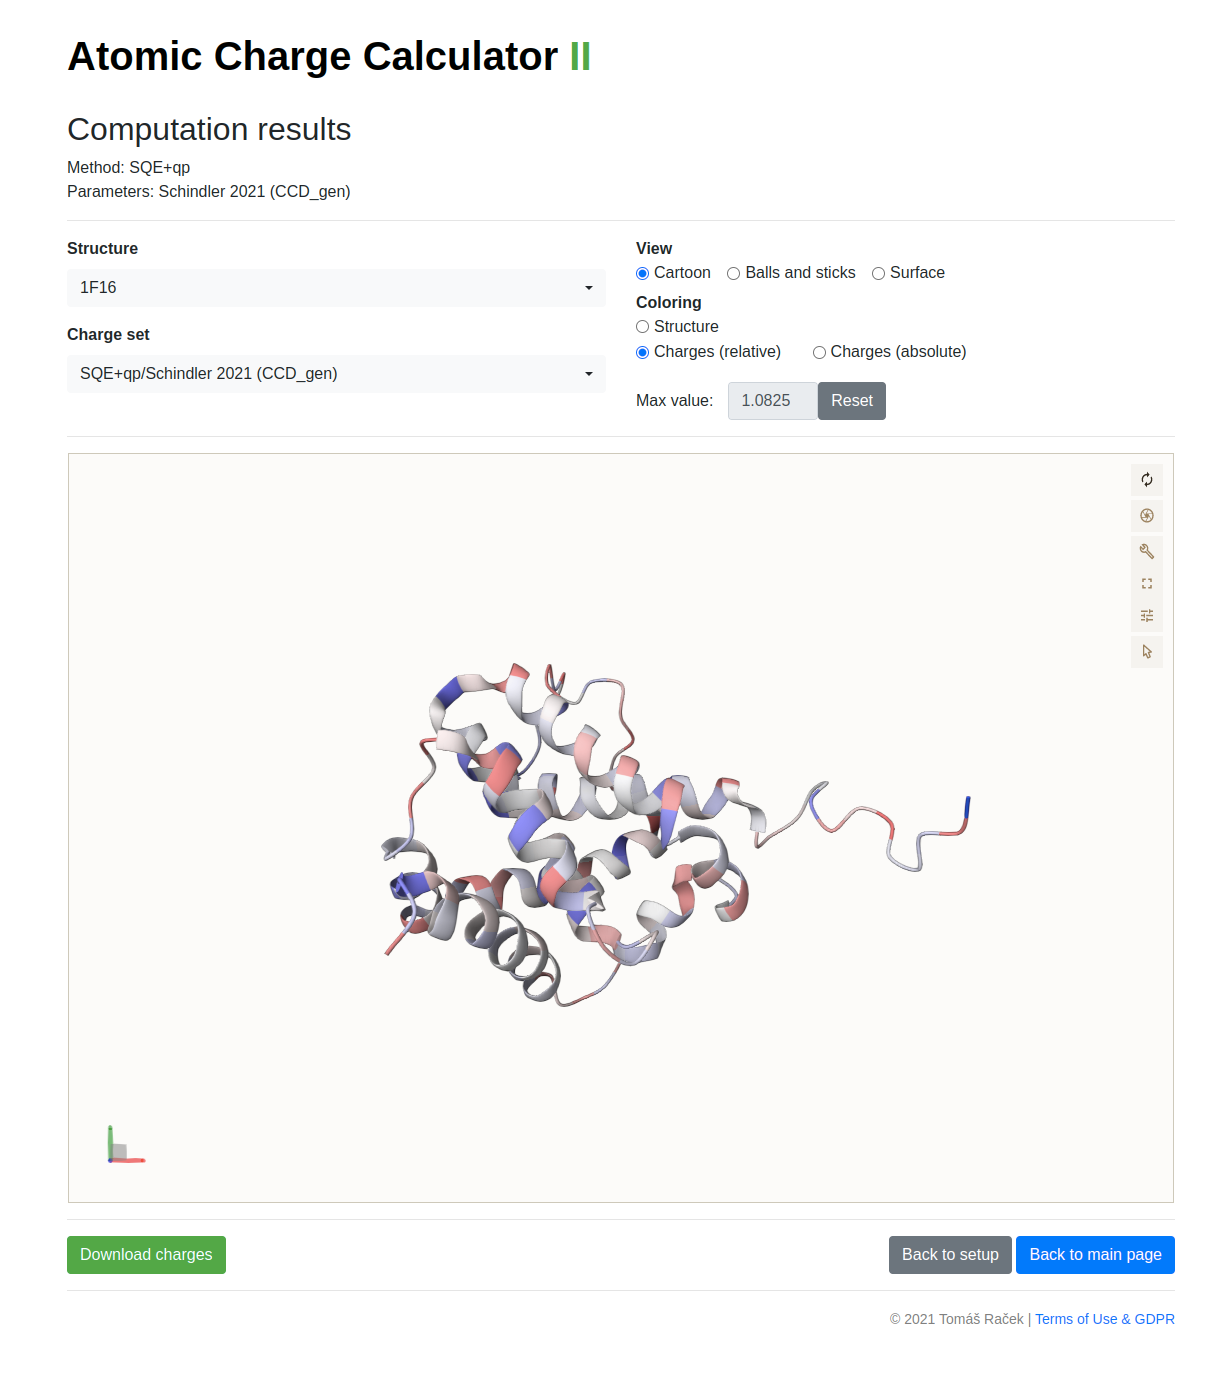
\includegraphics[width=\textwidth]{figures/results-full.png}
  \end{center}
  \caption{Updated result page for the ACC~II application.}
  \label{fig:result_page}
\end{figure}

Finally, the user can download all the output files generated by the backend in a ZIP archive by clicking the \textit{Download charges} button. Figure \ref{fig:output_dir_structure} shows the directory structure of the ZIP archive. The \texttt{cif} directory contains mmCIF files for each structure with all the charge sets. The name of each mmCIF file is the same as the name of the corresponding structure. The names of each file in the \texttt{txt}, \texttt{mol2}, and \texttt{pqr} directories are prefixed with the name of the structure and the name of the parameters used in the calculation for the given charge set.

\noindent
\begin{figure}[h]
  \begin{minipage}[t]{10cm}
    \dirtree{%
    .1 {charges} .
     .2 {cif} .
      .3 {1f16.fw2.cif} .
     .2 {mol2} .
     .2 {pqr} .
      .3 {1f16-EEM\_00\_NEEMP\_ccd2016\_npa.pqr} .
      .3 {1f16-SQEqp\_10\_Schindler2021\_CCD\_gen.pqr} .
     .2 {txt} .
      .3 {1f16-EEM\_00\_NEEMP\_ccd2016\_npa.txt} .
      .3 {1f16-SQEqp\_10\_Schindler2021\_CCD\_gen.txt} .
   }
   \end{minipage}\hfill
\caption{Directory structure of the output ZIP archive.}
\label{fig:output_dir_structure}
\end{figure}

\newpage

% * ✅
\chapter{αCharges}
\label{chapter:alphacharges}

αCharges (AlphaCharges) is a web application for calculating partial atomic charges for structures from AlphaFoldDB \cite{varadi2021alphafold}, a database of protein structures predicted by AlphaFold2 \cite{jumper2021alphafold}. The αCharges application protonates the protein structures (i.e., adds hydrogens) and calculates the partial atomic charges for the structures by the SQE+qp \cite{schindler2021sqe} empirical method. \cite{schindler2023alphacharges}

During the development of the αCharges application, the Mol* viewer was incorporated into the application to visualize the calculated partial atomic charges. The creators of the AlphaCharge application requested two additional features: a color theme for coloring the structure by the pLDDT confidence score and a page for visualizing problematic atoms in the structure.

The following sections describe the changes made to the Mol* viewer to support the αCharges application and implement the new features.

% * ✅
\section{Integration of the the Mol* viewer}

The αCharges application shares the architecture with the ACC~II application. The frontend is written in Javascript with the Bootstrap framework, and the backend is written in Python and uses the Flask framework. \cite{schindler2023alphacharges} This shared architecture allowed the integration of the Mol* viewer into the αCharges application with minimal adjustments. As with the ACC~II application, the Mol* viewer is incorporated into the result page by initializing the plugin viewer, loading the mmCIF file generated by the backend, and mounting the controls for managing the viewer.

% * ✅
\section{Coloring by pLDDT confidence score}

AlphaFold2 generates a confidence score for each residue in the predicted protein structures using a measure called pLDDT. The confidence score ranges between 0 and 100, where higher values indicate higher confidence levels. \cite{varadi2021alphafold} The AlphaFoldDB includes the confidence scores and predicted protein structures in the mmCIF file format. These confidence scores are stored in the mmCIF file under the following categories \cite{mmcif_dictionary}:

\begin{itemize}
  \item \texttt{\_ma\_qa\_metric} - contains details of the metrics use to assess model quality.
  \item \texttt{\_ma\_qa\_metric\_local} - contains information about the local quality scores calculated at the residue-level.
  \item \texttt{\_ma\_qa\_metric\_global} - contains information about the global quality scores calculated at the model-level.
\end{itemize}

The Mol* library supports coloring structures by the pLDDT confidence score. Figure \ref{fig:alphafold-coloring} shows the structure of a protein colored by the pLDDT confidence score. The coloring is based on the pLDDT confidence score of each residue. The confidence score of each residue is mapped to a set of colors, ranging from orange (low confidence) to dark blue (very high confidence).

\begin{figure}[htbp]
  \begin{center}
    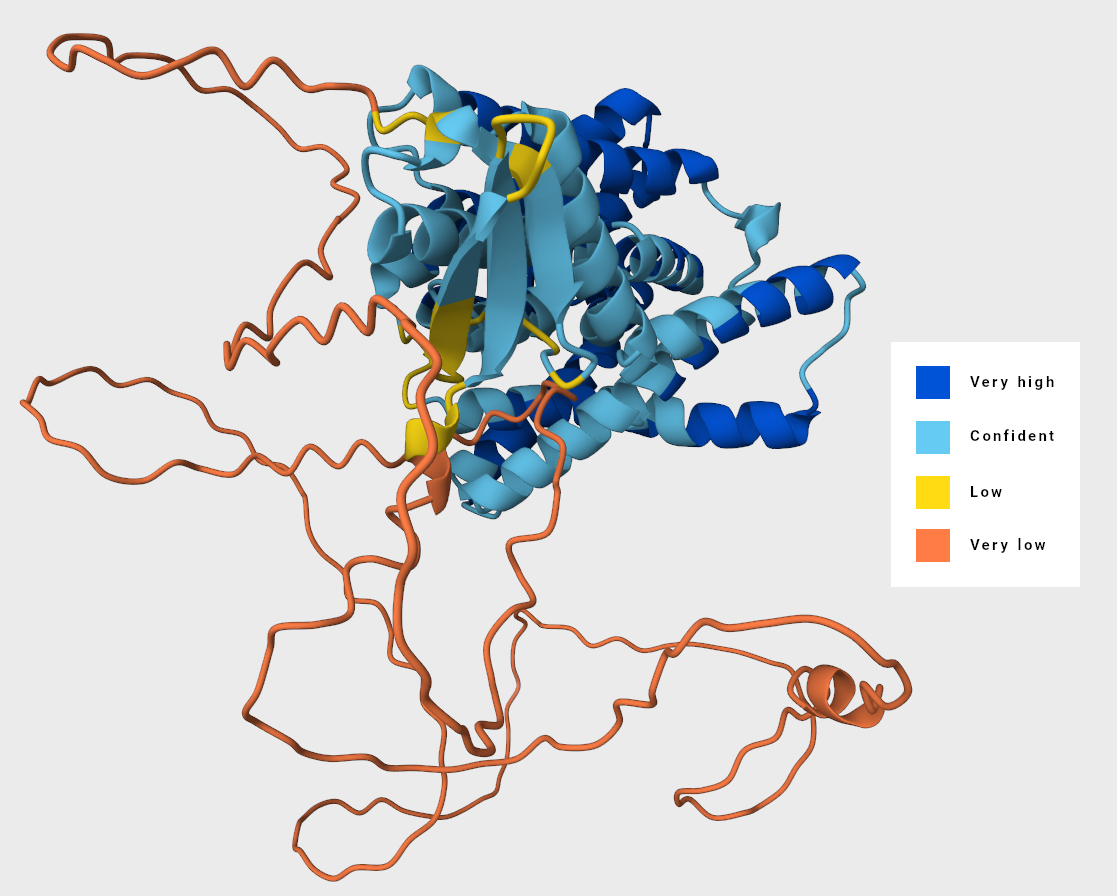
\includegraphics[width=7cm]{figures/alphafold_coloring.png}
  \end{center}
  \caption{Coloring of a protein structure by the pLDDT confidence score.}
  \label{fig:alphafold-coloring}
\end{figure}

To incorporate this coloring into αCharges, the backend of the application was extended to include the confidence scores in the output mmCIF file. This mmCIF file is sent to the frontend where it is loaded into the Mol* viewer. The αCharges application adds a new control to the result page for switching to the pLDDT color theme. Figure \ref{fig:alpha-charges-results} shows the result page of the αCharges application and highlights the new coloring control.

\begin{figure}[htbp]
  \begin{center}
    \includegraphics[width=\textwidth]{figures/alpha-charges-results.png}
  \end{center}
  \caption[Result page of the αCharges application.]{Result page of the αCharges application. The control for switching to the pLDDT color theme is highlighted in red.}
  \label{fig:alpha-charges-results}
\end{figure}

% * ✅
\section{Problematic structure page}

The αCharges application cannot calculate the partial atomic charges for all protein structures. The AlphaFold2 algorithm can incorrectly predict some structures or the application can fail to protonate the structure. \cite{schindler2023alphacharges} In such instances, the application automatically redirects the user to an error page, which displays the problematic structure in the Mol* viewer and an error message.

The error message is generated by the backend and contains a description of the error together with a list of each atom in the problematic structure that caused the error. When the user hovers over an atom in the list, a pop-up text is displayed explaining the probable cause of the error for the given atom. Figure \ref{fig:wrong_structure_text} shows the error message for a structure wrongly predicted by AlphaFold2 and the explanation as to why the atom \textit{GLN 33 CD} was wrongly predicted.

\begin{figure}[htbp]
  \begin{center}
    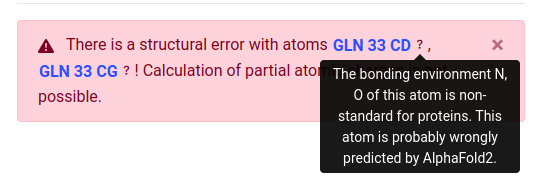
\includegraphics[width=7cm]{figures/wrong_structure_text.png}
  \end{center}
  \caption{Explanation of calculation error for atom \textit{GLN 33 CD}.}
  \label{fig:wrong_structure_text}
\end{figure}

Additionally, when the user clicks on an atom in the list, the Mol* viewer is focused on the atom. This allows the user to inspect the problematic atom in the structure. Figure \ref{fig:wrong_structure_focus} shows the Mol* viewer focused on the atom \textit{GLN 33 CD} of the problematic structure Q55GB6 from AlphaFoldDB.

\begin{figure}[htbp]
  \begin{center}
    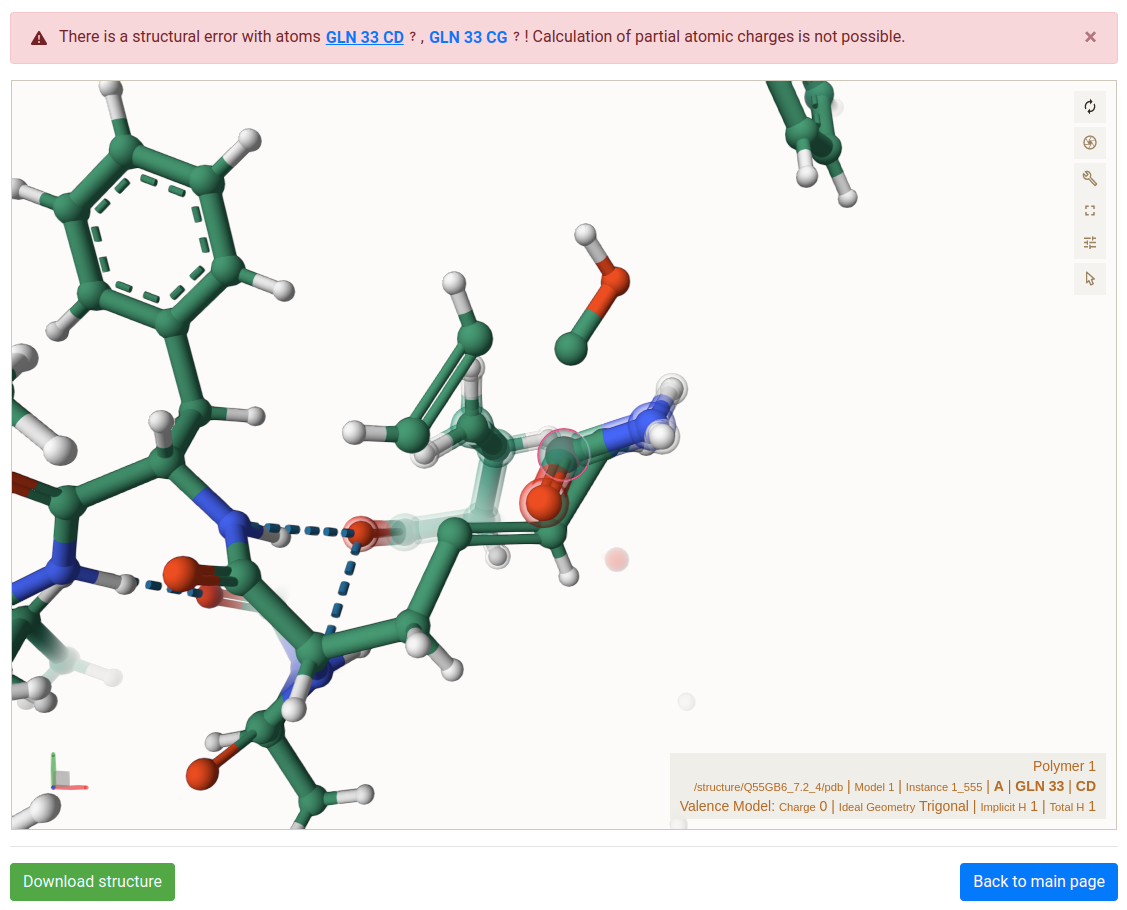
\includegraphics[width=\textwidth]{figures/wrong_structure_focus.png}
  \end{center}
  \caption{Focus on the atom GLN 33 CD.}
  \label{fig:wrong_structure_focus}
\end{figure}

\newpage

% * ✅
\chapter*{Conclusion}
\markright{\textsc{Conclusion}}
\addcontentsline{toc}{chapter}{Conclusion}

This thesis aimed to advance the field of computational chemistry by providing researchers with a modern visualization of partial atomic charges in Mol* and by expanding the capabilities of the Atomic Charge Calculator II and αCharges web applications.

We successfully extended the capabilities of the Mol* viewer to include the visualization of partial atomic charges. We incorporated the extended Mol* viewer into the Atomic Charge Calculator II and αCharges web applications.

We further enhanced the Atomic Charge Calculator II application with support for multiple calculations for a single request and implemented a new page for the αCharges web application for visualizing problematic atoms.

These advancements provide researchers with enhanced visualization capabilities and user interfaces for calculating and analyzing partial atomic charges. The significance of these improvements to the field of computational chemistry is substantiated by their contribution to a publication in the Nucleic Acids Research journal.

All source code developed in this work is available in the attachments and on GitHub. Links to the GitHub repositories can be found in Appendix \ref{appendix:source-code}. The extension to the Mol* viewer is also available in the official Mol* repository. 

\printbibliography[heading=bibintoc]

\renewcommand\appendixname{Appendix}
\newpage

% * ✅
\begin{appendices}
  \chapter{Source code}
  \label{appendix:source-code}
  All source code can be found in the attachments and on GitHub. Below are the links to the GitHub repositories:
  \begin{itemize}
    \item αCharges: \\
    \url{https://github.com/sb-ncbr/AlphaCharges}
    \item Atomic Charge Calculator II: \\
    \url{https://github.com/sb-ncbr/AtomicChargeCalculator2}
    \item ChargeFW2: \\
    \url{https://github.com/sb-ncbr/ChargeFW2}
    \item Mol* viewer plugin: \\
    \url{https://github.com/MergunFrimen/molstar-partial-charges}
  \end{itemize}

  \chapter[αCharges paper]{αCharges: partial atomic charges for AlphaFold
  structures in high quality}
  \label{appendix:alpha-charges}
  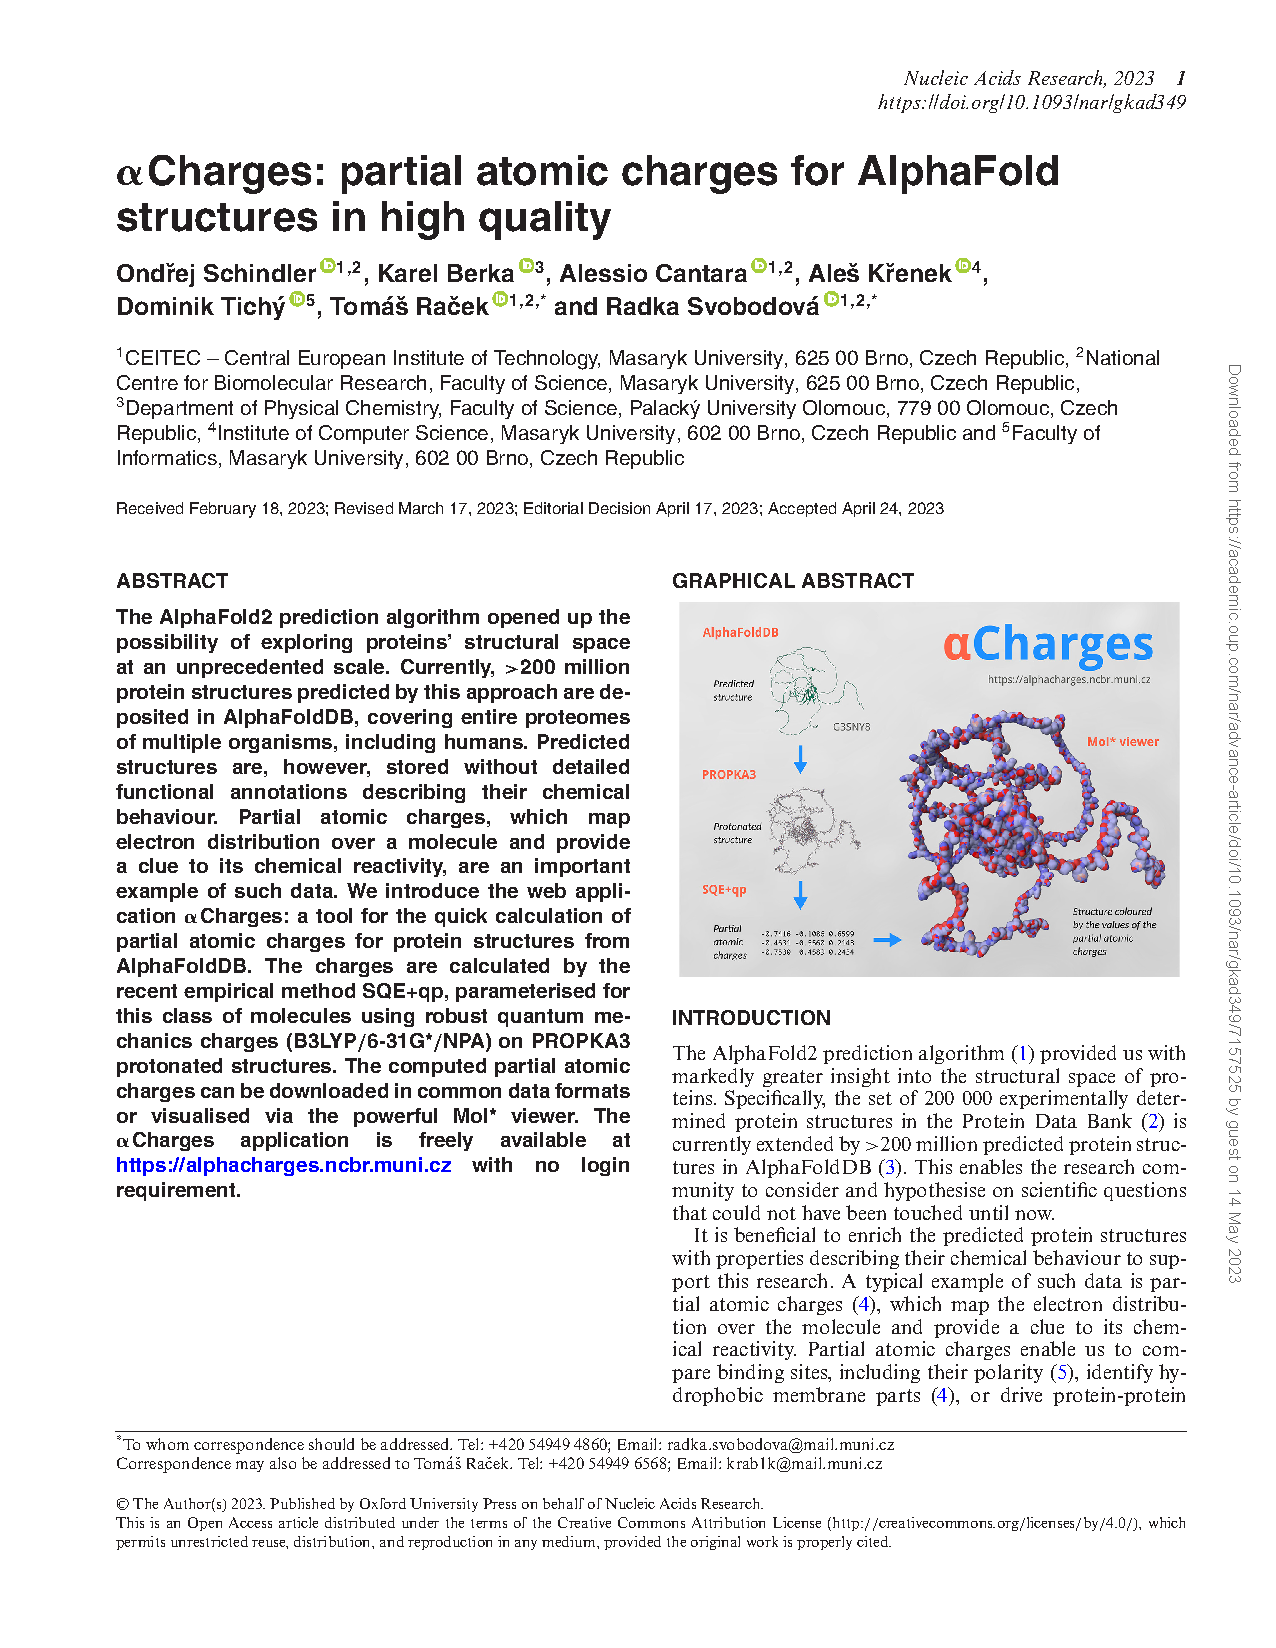
\includepdf[pages=-,offset=0cm 0cm]{figures/alphachargespaper.pdf}
\end{appendices}

\end{document}